%=======================================================================
% CSE465 Final Report --- North South University
%
% BUILD: pdfLaTeX on Overleaf. Order: pdflatex -> bibtex -> pdflatex x2
%
%======================================================================
\documentclass[journal,onecolumn]{IEEEtran}

\usepackage{graphicx}
\usepackage{amsmath}
\usepackage{amssymb}
\usepackage{booktabs}
\usepackage{multirow}
\usepackage{array}
\usepackage{url}
\usepackage[hidelinks]{hyperref}

\newcommand{\best}[1]{\textbf{#1}}
\newcommand{\notrun}{\textsc{not run}}
\newcommand{\notrec}{\textsc{not recoverable}}

\setcounter{topnumber}{4}
\setcounter{bottomnumber}{3}
\setcounter{totalnumber}{6}
\renewcommand{\topfraction}{0.92}
\renewcommand{\bottomfraction}{0.9}
\renewcommand{\textfraction}{0.05}
\renewcommand{\floatpagefraction}{0.7}

\begin{document}

\title{Auditing the Score Before the Model: Corrected Evaluation
Baselines and a Pre-Registered Negative Result for Respiratory Sound
Classification on ICBHI 2017}

\author{Barshon~Basak,~Asif~Mahbub,~Sami~Uddin,~and~Farhana~Rahman%
\thanks{The authors are with the Department of Electrical and Computer
Engineering, North South University, Dhaka, Bangladesh.}%
\thanks{The authors thank Dr.~Riasat Khan for supervising this work.}}

\maketitle

%=======================================================================
\begin{abstract}
Respiratory sound classification is judged almost everywhere on one public lung sound
benchmark, and almost every system is ranked by a single headline score. This study set out
to build a better classifier and arrived at a prior question: how much of that score
belongs to the model, and how much to the way it was measured. We audited our own
pipeline of 39 experiments and found five faults in the measurement itself, each recovered
from a stored prediction table. A wrongly averaged score
variant inflated 20 runs by 9.5 points on average and 22 at worst. A split loader that
silently fell back to a patient identifier rule produced a test partition of 11 patients
while recording itself as the official one, worth almost 9 points alone. The published
partition assigns recordings instead of patients, so two patients sit on both sides, though
repairing that leak moves the score by four tenths of a point. One recording carries a device
suffix the released audio does not, so a naive join drops it silently. Choosing the saved
model by training loss rather than by the challenge score costs 7 to 10 points across three
seeds. Under a corrected protocol we segment every breathing cycle, convert it to a log scaled
spectrogram, and train one lightweight convolutional network and three pretrained vision
transformers, reporting accuracy, precision, recall, sensitivity, specificity, parameter
count, size and training time for each, with and without spectrogram masking.
A fourth transformer, pretrained on general audio before the audit, stored no prediction
table and is reported as unrecoverable. The best model is then examined
with a twelve row ablation study, a three seed noise floor, paired patient level tests, and
explainable artificial intelligence. The contribution is a measurement, not a mechanism.
\end{abstract}

\begin{IEEEkeywords}
Ablation study, convolutional neural network, data augmentation, evaluation protocol,
explainable artificial intelligence, ICBHI 2017, label reliability, pre-registration,
reproducibility, respiratory sound classification, transfer learning, vision transformer.
\end{IEEEkeywords}

%=======================================================================
\section{Introduction}
\label{sec:intro}

A stethoscope is still the first instrument a doctor reaches for when examining a
patient presenting with a respiratory condition. The crackles and wheezes get drowned
by the sound of the heart beating and environmental noises. The diagnosis still varies
widely from one doctor to the next. The ICBHI 2017 Respiratory Sound
Database~\cite{rocha2019icbhi} is a standard resource to consult when embarking on this
journey to automate respiratory detection with machine learning. This problem was
selected because the benchmark is mature. A brand-new architecture is not the goal, but a
mature benchmark is a reasonable setting in which to ask a different kind of question. Do the scores the
field reports on this corpus mean what everybody takes them to mean? We started by
asking it of ourselves.

\subsection{Literature Review}
\label{subsec:lit}

Yu \emph{et al.}~\cite{electronics2025review} have reviewed 135 technical publications
built on this database. They separated the tasks into two. To recognise the patient's
pathological state, where many systems exceed 98 percent accuracy. To categorise the
adventitious sound in a single cycle. Severe class imbalance makes the second task much
more difficult. They suggest using the data surrounding the audio more effectively and
creating models that are easier to understand. Recent work is driven in that direction.
Since around 2021, progress has come more from better pre-training than from a better
architecture. Convolutional systems pretrained on ImageNet~\cite{deng2009imagenet}
plateau near 0.56 on the official challenge metric~\cite{respirenet2021}. Transformers
pretrained on AudioSet~\cite{gemmeke2017audioset} score five to nine points
higher~\cite{bae2023patchmix,bts2024,pafa2025}. Suma \emph{et al.}~\cite{suma2025mtl}
targets both tasks at once, with a single-input, multi-output network over
mel-frequency cepstral coefficients. They compare four backbones. MobileNet performs
best with 74 percent on sounds and 91 percent on diseases. They never state which
partition those numbers are on. That is the first sign of the problem this paper
addresses. Two 2025 fusion systems~\cite{adffnet2025,bspc2025fusion} report gains of
roughly one point, the scale at which the measurement questions below start to matter.

Bae \emph{et al.}~\cite{bae2023patchmix} fine-tuned an Audio Spectrogram
Transformer~\cite{gong2021ast} with a patch-mixing contrastive objective and achieved
0.6237. Niizumi \emph{et al.}~\cite{frozenfm2025} froze the audio foundation model
entirely, trained only a linear probe, and still achieved 0.5938. That is above several
fully fine-tuned convolutional systems. Most of the useful information sits in the
pretrained representation, not the fine-tuning, provided the pretraining was on audio.
Moummad and Farrugia~\cite{scl2023} achieved 0.5755 using a small CNN and contrastive
pretraining on metadata. Nguyen and Pernkopf~\cite{nguyen2022cotuning} add that the
transfer from ImageNet to spectrograms is fragile. It needs regularisation. Kim \emph{et
al.}~\cite{kim2025metadata} pushed the metadata idea furthest. They reached a
conclusion we had to confront directly. They evaluated recording devices, chest
location, sex, and age as sources of domain shift. They used the most informative
combinations to guide a supervised contrastive objective and identified
recording-condition bias as a primary limiting factor for models trained on this
corpus. Section~\ref{subsec:dataset} reports what we found when we went looking for
that axis in the data itself.

To examine the reasons behind a prediction, concept bottleneck
models~\cite{koh2020cbm} filter it using human-defined concepts. This is appealing
since wheezes and crackles have physical definitions. This was our original plan.
Karim \emph{et al.}~\cite{karim2024mosquito} combined vision transformers with OpenMax
rejection. We reimplemented that as our open-set baseline. Knowledge distillation with
a teaching assistant~\cite{pavel2024kd} gave us the compression arm. Yang \emph{et
al.}~\cite{yang2024ood} has done the vocabulary separating out-of-distribution
detection from open-set recognition. Kejriwal \emph{et al.}~\cite{kejriwal2024owl} has
done the staged open-world protocol. Cho and Lee~\cite{cho2025openset} are the only
group found to have performed open-set recognition on respiratory audio. They reported
an improvement over a semi-supervised baseline, not an absolute score. Cruz \emph{et
al.}~\cite{cruz2025owl} surveyed what the open-world field still has not solved. They
group the open problems into three areas. The theory of novelty, the design of agents,
and their evaluation. The third area aligns with us. They name inconsistent evaluation
metrics as an unresolved issue.

Tzeng \emph{et al.}~\cite{tzeng2025jmir} had seven senior physicians blindly annotate a
quarter of the ICBHI test set. On clean audio, they reached an ICBHI score of 47.77
percent, with a sensitivity of 23.23 percent, and a mean self-rated confidence of 2.88
out of 5. Melbye \emph{et al.}~\cite{melbye2016kappa} had twelve physicians classify
twenty reference recordings. The agreement fell below $\kappa = 0.40$ for detailed
descriptions. It rose to 0.62 and 0.59 when crackles and wheezes were collapsed to a
simple presence. Huang \emph{et al.}~\cite{huang2024crackles} report a larger clinical
archive with agreement on wheezes being very high ($\kappa = 0.948$) and agreement on
crackle being only moderate ($\kappa = 0.516$). The three studies disagree on the
level. They do agree on the shape, that crackle labels are far less reliable than
wheeze labels. Reliability falls sharply as the description gets finer. Bikku \emph{et
al.}~\cite{scirep2025cnnrnn} fused a convolutional encoder with a recurrent one over
mel-spectrograms drawn from two corpora. They map crackles to pneumonia, wheezes to
obstructive disease. They explain the result with gradient, Shapley, and local
surrogate methods, reporting 94.0 percent accuracy under five-fold cross-validation.
The explanations align with the same cycle labels that the three studies characterised
earlier. The partition is not the official one. The number cannot be read against the
systems in the first block. Both observations shaped how we report our own
interpretability results in Section~\ref{subsec:xai}.

\subsection{Gaps in the Related Work}
\label{subsec:gaps}

Reading the two groups side by side exposed four gaps we could act on.

The reported score is treated as a characteristic of the model. Papers from the first
group report their composite numbers and compare them with those of other papers. A
few of them state the circulating definition they used. The description of the
partition is often vague or non-existent. The multi-task study does not name any.
Five-fold cross-validation is reported in the convolutional-recurrent study, which
can't be compared to the official split figures next to it. We could not find an ICBHI
paper that ablates its evaluation protocol the way it ablates its architecture. Our own
audit shows the protocol is worth more than any architectural choice we made.

The official split is assumed to be independent of the patient, but it is not. The
published file assigns recordings, not patients. Two patients have recordings on both
sides. That is a validity fault that no paper we read mentions.

The reference standard is never characterised. The first group validates models
against ICBHI's cycle labels. The second shows that those labels are reproduced by
trained physicians at only 47.77 percent, with agreement ($\kappa$) well below 0.40 for
fine distinctions. A detector scored against a reference standard of unknown
reliability produces a number of unknown meanings.

We could not find a paper that set a validity threshold in advance, ran a test against it, and reported a failure. Without that, a reader cannot tell how many attempts a reported success survived.

\subsection{Our Work}
\label{subsec:ourwork}

We began with the goal of open-world multi-task design. It had a shared spectrogram
backbone, one head for the four sound-event classes, and one head for disease. A
bottleneck of physics-derived acoustic concepts sat in between. We set a threshold that
the crackle and wheeze labels from ICBHI must be replicated by the extractors with an
area under the curve of at least 0.65, with an interval that excludes chance. We
checked once per run on the test partition. We committed to two attempts before
starting. Wheeze failed at 0.5729, then at 0.5340, and crackle failed at 0.5506, then
at 0.5580. We stopped here because the attempts were unsuccessful per the threshold.

We looked back to see if we could measure anything. Five flaws in our own assessment
were discovered by the audit. The five faults are set out in Section~\ref{subsec:faults}.
Our headline number changed from 0.7077 to 0.5602 once they were fixed. The difference
is 0.1475. It outweighs the impact of ImageNet pretraining. It is more than the
augmentation effect, and it is more than the difference between our strongest and
weakest backbones. We provided a measurement instead of a mechanism. It includes a
revised methodology, baselines generated using it, and tools that enable another person
to identify every flaw.

We then rebuilt the model side under that protocol. We trained one ImageNet-pretrained
convolutional network. We trained three ImageNet-pretrained vision
transformers~\cite{dosovitskiy2021vit,liu2021swin,touvron2021deit}. All four models
used identical inputs. All four used identical schedules. Each model had two runs, one
clean and one with SpecAugment~\cite{park2019specaugment}.

A fourth transformer, an Audio Spectrogram Transformer~\cite{gong2021ast} pretrained on
AudioSet, had been run earlier in the project. It predates the audit. It stored no
prediction table. Its challenge-metric score cannot be recovered. Section~\ref{subsec:ast}
reports that gap directly. It does not repair the gap. This gap is the clearest
illustration of the paper's own argument.

The best model, MobileNetV2~\cite{sandler2018mobilenetv2} with SpecAugment, underwent a
twelve row ablation study. It went through a three-seed noise floor test. It went through
paired patient-level tests. It went through gradient-based
attribution~\cite{selvaraju2017gradcam}. It went through occlusion-based
attribution~\cite{selvaraju2017gradcam}. Every transformer lost to the convolutional
baseline. The largest transformer collapsed to the majority class. We report that
rather than tuning until it stops being true.

Finally, we returned to the concept question with a fairer instrument. It refuted the
explanation we had begun to prefer. See Section~\ref{subsec:ceiling}.

The novelty here is not a layer. It is not a loss. It is five things.

\begin{itemize}
\item We ablate the evaluation protocol itself. We have not seen this done on this
benchmark.
\item We treat the checkpoint selection rule as a first-class pipeline component. It is
worth more than pretraining. It is worth more than augmentation.
\item We use a measured run-to-run noise floor. It works as an admissibility threshold
for every ablation delta we report.
\item We set a pre-registered gate. It failed. We then made a pre-registered ceiling
estimate. That estimate refuted our own account of why the gate failed.
\item We ran an attribution analysis. It contradicts the story the score tells. It
directly motivated one of the ablation rows.
\end{itemize}

The remainder of this paper is organised as follows. Section~\ref{sec:system} describes the
proposed system: the corpus and its partitions in Section~\ref{subsec:dataset}, the
preprocessing chain in Section~\ref{subsec:preprocessing}, the four backbones and their training
schedules in Section~\ref{subsec:models}, and the evaluation metrics and the pre-registered gate
in Section~\ref{subsec:metrics}. Section~\ref{sec:results} reports every numerical result,
opening with the evaluation audit in Section~\ref{subsec:faults}, followed by the main
comparison, model cost, augmentation, the best model in detail, the statistical analysis, the
ablation study, the extension experiments, the concept gate and its ceiling estimate, the
comparison against a physician, the interpretability analysis, and finally the comparison
against published systems in Section~\ref{subsec:comparison}. Section~\ref{sec:conclusion}
draws the conclusions and states three directions for future work.

%=======================================================================
\section{Proposed System}
\label{sec:system}

All numerical results are saved for Section~\ref{sec:results}. The numbers here are
characteristics of the data. The entire system is depicted in Fig.~\ref{fig:flowchart}
below. Additionally, it shows the locations of each of the five faults listed in
Section~\ref{subsec:faults}.

\begin{figure}[!t]
\centering
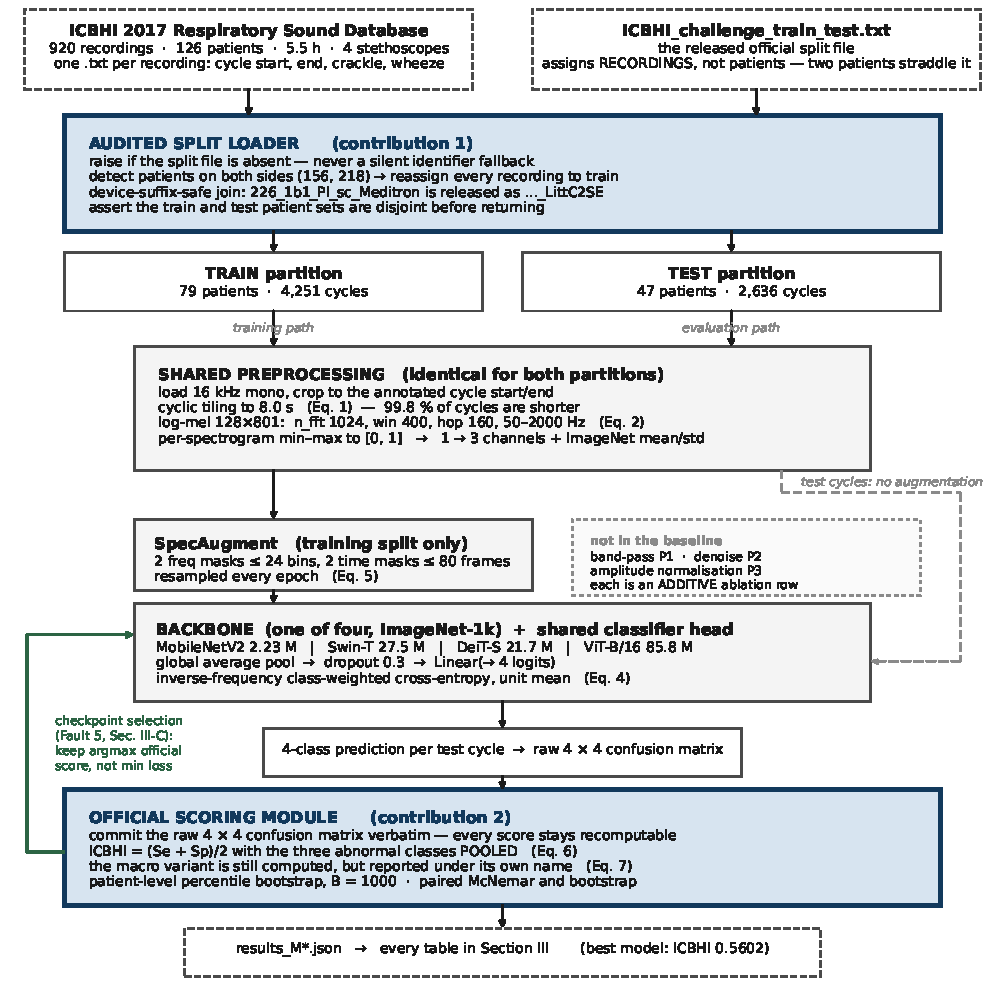
\includegraphics[width=0.38\linewidth]{figures/fig_flowchart.pdf}
\caption{Flowchart of the complete system. Audio is segmented into annotated respiratory
cycles, standardised in length, converted to a log-mel spectrogram and classified into four
sound-event classes. The split loader, the metric definition and the checkpoint selection
rule are treated as pipeline components with their own ablation rows rather than as fixed
infrastructure.}
\label{fig:flowchart}
\end{figure}

\subsection{Dataset}
\label{subsec:dataset}

We use the ICBHI 2017 Respiratory Sound Database~\cite{rocha2019icbhi} from its public
release. It includes 920 recordings from 126 patients, annotated per respiratory cycle
with a start time, an end time, a crackle flag, and a wheeze flag. Combining the two
flags gives us the four sound-event classes used throughout. They are labelled as
Normal, Crackle, Wheeze, and Both, over 6,898 annotated cycles with a median length of
2.42~s. We standardise that to an 8.0~s network input. Recordings were captured with
four stethoscopes at several chest locations and at mixed sample rates. We resample it
all to 16~kHz mono.

Two structural facts about the corpus shaped the project and are worth stating before
any results. Each patient carries a single diagnosis label. Those labels are extremely
imbalanced: COPD alone covers 64 of the 126 patients, 83.3 percent of all cycles. That
is why the disease side of our original two-head design was eventually dropped from the
headline. Only 4 patients (112, 158, 218, and 226) were recorded on more than one
device. Device identity is almost perfectly confounded with patient identity. Kim
\emph{et al.}~\cite{kim2025metadata} identify recording-condition bias as a primary
limiting factor for models trained here: that is worth stating plainly. The axis they
show matters is one this corpus cannot measure from the inside. Separating the device
from the patient would require patients to be recorded on several devices, and there
are only four. It is a reason to take their cross-dataset approach seriously, not a
reason to doubt it.

Table~\ref{tab:partitions} presents the three partitions used in this paper, along with
the class composition of each. The published split file assigns recordings, not
patients. Patients 156 and 218 have recordings on both sides. Our corrected partition
moves every recording of a leaking patient into the training side. That is the
conservative direction. The test side is then guaranteed to contain no patient the
model has trained on. The repair costs 12 of 381 test recordings. It moves the ratio
from 58.6/41.4 to 59.9/40.1, marginally closer to the nominal 60/40 than the published
file itself. All new results in this paper are on the corrected partition. The other
two partitions appear only where a comparison demands it, always by name.

On the corrected test partition, the Both class holds 86 cycles against 1,560 Normal.
This shows how severe the imbalance is. That is why every model here trains with an
inverse-frequency weighted loss, (\ref{eq:weights}). It is also why accuracy is a
misleading headline on this corpus: a classifier that always predicts Normal attains the
majority-class accuracy of the partition while detecting nothing, which
Section~\ref{subsec:main} quantifies against the trained models.

\begin{table}[!t]
\centering
\caption{The three partitions used in this paper with the class composition of each, computed
from the ICBHI annotation files and cross-checked against the committed confusion matrix of the
corresponding run. Spectrogram masking operates in place and adds no samples, so the augmented
training total equals the clean one.}
\label{tab:partitions}
\footnotesize
\begin{tabular}{llrrrrrrrr}
\toprule
Partition & Subset & Normal & Crackle & Wheeze & Both & Total & Aug.\ total & Patients & Rec. \\
\midrule
Whole corpus & --- & 3{,}642 & 1{,}864 & 886 & 506 & 6{,}898 & --- & 126 & 920 \\
\midrule
\multirow{2}{*}{\best{Corrected (ours)}}
 & Train & 2{,}082 & 1{,}247 & 513 & 420 & 4{,}262 & 4{,}262 & 79 & 551 \\
 & Test  & 1{,}560 & \phantom{0,}617 & 373 & \phantom{0}86 & 2{,}636 & --- & 47 & 369 \\
\midrule
\multirow{2}{*}{Published, verbatim}
 & Train & 2{,}063 & 1{,}215 & 501 & 363 & 4{,}142 & 4{,}142 & 77 & 539 \\
 & Test  & 1{,}579 & \phantom{0,}649 & 385 & 143 & 2{,}756 & --- & 49 & 381 \\
\midrule
\multirow{2}{*}{Identifier fallback}
 & Train & 3{,}387 & 1{,}700 & 848 & 471 & 6{,}406 & 6{,}406 & 115 & --- \\
 & Test  & \phantom{0,}255 & \phantom{0,}164 & \phantom{0}38 & \phantom{0}35 & \phantom{2,}492 & --- & \phantom{0}11 & --- \\
\bottomrule
\end{tabular}

\vspace{2pt}
\footnotesize The corrected partition reassigns the two leaking patients to training; the
published partition is the split file verbatim; the identifier-fallback partition is not a
design but a fault (Section~\ref{subsec:faults}). Two earlier backbone runs use a fourth
policy that instead \emph{drops} the leaking patients' training recordings and leaves the
published test set byte-identical, so their test row is the published test row. Pooling the
abnormal classes, the corrected test partition holds 703 crackle-positive and 459
wheeze-positive cycles, the denominators of every concept result in
Section~\ref{subsec:gate}. One recording named \texttt{226\_1b1\_Pl\_sc\_Meditron} in the
split file is released as \texttt{226\_1b1\_Pl\_sc\_LittC2SE}, so a stem join drops it and its
11 cycles; it is a training recording, which is why our pipeline indexes 4,251 training cycles
where the annotations hold 4,262.
\end{table}

\subsection{Dataset Preprocessing}
\label{subsec:preprocessing}

The chain is implemented once. Every stage is switchable. That lets the ablation in
Section~\ref{subsec:ablation} change one thing at a time. The execution order is:

\begin{enumerate}
\item Load and resample to 16~kHz mono.
\item Optionally band-pass filter with a zero-phase fourth-order Butterworth between
50 and 2000~Hz.
\item Segment into cycles at the annotated start and end times.
\item Standardise every cycle to 8.0~s by cyclic tiling, Eq.~(\ref{eq:tile}).
\item Optionally normalise each cycle to unit peak amplitude.
\item Optionally denoise by spectral gating at the 25th percentile, with an
over-subtraction factor of two.
\item Compute a log-mel spectrogram, Eq.~(\ref{eq:logmel}), with 128 mel bands, a
1024-point FFT, hop 160, and window 400, over 50 to 2000~Hz.
\item Rescale each spectrogram to the unit interval, Eq.~(\ref{eq:minmax}).
\item Replicate to three channels for the pretrained backbones.
\item Encode the label, Eq.~(\ref{eq:label}).
\item Handle imbalance in the loss, Eq.~(\ref{eq:weights}).
\item Apply spectrogram masking, Eq.~(\ref{eq:specaug}), to the training split only.
\end{enumerate}

Three of those stages are off in the reference configuration and are done
deliberately. They are band-pass filtering, denoising, and per-cycle amplitude
normalization. Turning any of them on in the reference would silently move the
baseline that every other ablation delta is measured against. Instead, they are
switched on one at a time, as rows \texttt{P1}, \texttt{P2}, and \texttt{P3} of
Table~\ref{tab:ablation}. Their deltas therefore read in the opposite direction to
every other row: a positive delta is a recommendation to adopt the stage.

The median cycle is 2.42~s, against an 8.0~s input. Almost every cycle has to be
extended. We tile rather than pad with silence. For a cycle $x$ of length $L$, and a
target of $N = T f_s$ samples:

\begin{equation}
\tilde{x}[n] = x[n \bmod L], \qquad n = 0,\dots,N-1,
\label{eq:tile}
\end{equation}

A longer cycle is cropped from the start. Tiling is common practice here. It repeats
the same acoustic event two or three times within a single input. It leaves a
discontinuity at each seam. Row \texttt{P4} tests the alternative for reasons provided
in Section~\ref{subsec:xai}. The tiled waveform is converted to a log-mel spectrogram.
$X[m,k]$ is the short-time Fourier transform. $H_j[k]$ is the $j$-th mel filter:

\begin{equation}
S[j,m] = 10\log_{10}\!\left(\frac{\sum_{k} H_j[k]\,\lvert X[m,k]\rvert^{2}}
{\displaystyle\max_{j',m'}\ \sum_{k} H_{j'}[k]\,\lvert X[m',k]\rvert^{2}}\right).
\label{eq:logmel}
\end{equation}

The maximum is per spectrogram, not global. That is itself a normalisation. It is why
the explicit rescaling that follows is nearly free in the ablation. That rescaling is a
min--max map to the unit interval:

\begin{equation}
\tilde{S} = \frac{S - \min S}{\max S - \min S + \epsilon}, \qquad \epsilon = 10^{-8}.
\label{eq:minmax}
\end{equation}

Labels come from the two annotation flags: $c$ is the crackle flag, $w$ is the wheeze
flag, both in $\{0,1\}$:

\begin{equation}
y = c + 2w \in \{0,1,2,3\} \;\equiv\; \{\text{Normal},\ \text{Crackle},\ \text{Wheeze},\ \text{Both}\}.
\label{eq:label}
\end{equation}

Imbalance is handled in the loss, not by resampling. That keeps the training
distribution identical across every model and ablation row. For class $c$, with $N_c$
of $N$ training cycles and $C = 4$, the raw inverse-frequency weight is renormalised to
unit mean:

\begin{equation}
w_c = \frac{N}{C N_c} \bigg/ \frac{1}{C}\sum_{c'=1}^{C}\frac{N}{C N_{c'}},
\qquad
\mathcal{L} = -\frac{1}{B}\sum_{i=1}^{B} w_{y_i}\log p_{i,y_i}.
\label{eq:weights}
\end{equation}

Without renormalisation, the loss scale moves with the class distribution. Ablation
rows that change the training set would then no longer be comparable to the reference.
SpecAugment~\cite{park2019specaugment} is applied only to training spectrograms, using
the same seed as the paired clean run. The two runs differ in exactly one thing:

\begin{equation}
\tilde{S}[j,m] \leftarrow 0 \ \ \text{for}\ j \in [f_0, f_0{+}f),\ f \sim \mathcal{U}[0,24],
\ \ \text{and}\ m \in [t_0, t_0{+}t),\ t \sim \mathcal{U}[0,80],
\label{eq:specaug}
\end{equation}

Two frequency masks, two time masks, per spectrogram.

\subsection{Applied Models}
\label{subsec:models}

Table~\ref{tab:models} lists every model, with its owner. The four backbones trained
under the corrected protocol share the same spectrograms, loss, partition, batch size
of 16, cap of 40 epochs, and seed 42. Anything else would turn the comparison into a
comparison of tuning effort. Only the classifier head is replaced. The two families do
differ in optimiser settings. We state that rather than smoothing it over. The
convolutional model employs Adam with a single learning rate of $5\times10^{-4}$,
dropout of 0.3, and gradient clipping of 5.0. The vision transformers use AdamW at
$10^{-4}$ on the backbone and $10^{-3}$ on the head, which is the conventional way to
fine-tune a pretrained transformer. Both use cosine annealing and weight decay of
$10^{-4}$. The ablation harness reuses the convolutional settings unchanged.

\begin{table}[!t]
\centering
\caption{Every model in this paper. The four backbones
of the first block take the same $128 \times 801$ log-mel input replicated to three
channels, and each was run twice, clean and with spectrogram masking.}
\label{tab:models}
\footnotesize
\begin{tabular}{llll}
\toprule
Backbone & Family & Pretraining & Protocol and role \\
\midrule
MobileNetV2~\cite{sandler2018mobilenetv2} & CNN & ImageNet & corrected partition \\
ViT-B/16~\cite{dosovitskiy2021vit} & Transformer & ImageNet-21k & corrected partition \\
Swin-T~\cite{liu2021swin} & Transformer & ImageNet & corrected partition \\
DeiT-S~\cite{touvron2021deit} & Transformer & ImageNet & corrected partition \\
\midrule
AST~\cite{gong2021ast} & Transformer & ImageNet + AudioSet & pre-audit; score \notrec \\
2D-CNN, 4 blocks & CNN & from scratch & alternative partition; reference \\
MobileNetV3-Small & CNN & ImageNet & alternative partition; reference \\
MobileNetV2 ensemble, $N{=}5$ & CNN & ImageNet & calibration carve-out; extension \\
\bottomrule
\end{tabular}

\vspace{2pt}
\footnotesize The Audio Spectrogram Transformer is the only audio-domain pretrained backbone in
the project and the only one of the four transformers run before the evaluation audit. It
committed no raw confusion matrix, so its challenge-metric score cannot be recomputed;
Section~\ref{subsec:ast} reports what does exist and treats the gap as evidence rather than as
an omission.
\end{table}

\subsection{Evaluation Metrics}
\label{subsec:metrics}

The ICBHI 2017 challenge metric pools the three abnormal classes against Normal. $M$ is
the $4\times4$ confusion matrix. Rows are the true class. Index 0 is Normal.

\begin{equation}
S_e = \frac{\sum_{i=1}^{3} M_{ii}}{\sum_{i=1}^{3}\sum_{j=0}^{3} M_{ij}},
\qquad
S_p = \frac{M_{00}}{\sum_{j=0}^{3} M_{0j}},
\qquad
\mathrm{ICBHI} = \frac{S_e + S_p}{2}.
\label{eq:official}
\end{equation}

A second definition circulates. It is the one our pipeline used before the audit. This
one is a macro average of per-class recall and per-class specificity:

\begin{equation}
\mathrm{ICBHI}_{\mathrm{macro}} = \frac{1}{2}\left(
\frac{1}{C}\sum_{c=0}^{C-1}\mathrm{Recall}_c +
\frac{1}{C}\sum_{c=0}^{C-1}\mathrm{Specificity}_c \right).
\label{eq:macro}
\end{equation}

The two are not close. Each per-class specificity in that macro formula counts true
negatives drawn from the other three classes. A rare class, such as Both, scores near
0.95 almost regardless of whether the model ever predicts it. Alongside the challenge
metric, we report accuracy, macro precision, macro recall, macro F1, parameters, size,
and training time for every model. Confidence intervals resample patients, not cycles,
2,000 times. Two configurations are compared by paired patient-level bootstrap. Where
per-cycle predictions exist for both, they are also compared by McNemar's test. The
concept-validity gate of Section~\ref{subsec:gate} was fixed before it was run. A
concept passes if:

\begin{equation}
\mathrm{AUROC} \geq 0.65 \quad\text{and}\quad \text{the 95 percent DeLong interval excludes } 0.5,
\label{eq:gate}
\end{equation}

The interval is computed by the DeLong method~\cite{delong1988auc}. The 0.65 floor is
part of the rule for a reason. An earlier version required only that the interval
exclude chance. At $n \approx 2{,}600$, that is satisfied at an AUROC of 0.52:
significant, and useless. A gate that cannot fail is not a gate.

%=======================================================================
\section{Results and Discussion}
\label{sec:results}

In this section we present the results of the applied models for respiratory sound
classification. The convolutional runs, the three seed replicates and three of the preprocessing
ablation rows were trained on Kaggle and Google Colab with an NVIDIA Tesla T4 (16~GB). The
transformer runs and the remaining ablation rows were trained on a local workstation with an
NVIDIA GeForce RTX 4050 Laptop GPU (6~GB). Both setups used PyTorch 2.10 and CUDA 12.8.

This study reports 39 runs in total. The main comparison uses four backbones,
and each of them was trained twice, once with spectrogram masking and once without. Alongside
them we ran two more convolutional models as alternatives, MobileNetV3-Small and a 2D-CNN
trained from scratch, and one audio-pretrained transformer early in the project. The rest are
nine extension experiments, twelve ablation rows, three seed replicates of one configuration and
two concept-gate runs. Eight runs did not converge to a usable model; those runs and
concept-gate results are reported alongside the other outcomes in
Table~\ref{tab:allruns} and Sections~\ref{subsec:extensions} and~\ref{subsec:gate}.

Each run writes one result file that stores the run configuration, the raw $4\times4$ confusion
matrix, the per-epoch training history and the efficiency record. Every value we report in this
section was read from one of these files or recomputed from one. The Audio Spectrogram
Transformer of Section~\ref{subsec:ast} is the only exception, because we trained it before we
made this a rule, and we flag it everywhere it appears. Section~\ref{subsec:faults}
prices the evaluation audit, and Table~\ref{tab:partitions} defines the corrected
partition named throughout this section.

\subsection{Evaluation Audit}
\label{subsec:faults}

We audited the 39 committed runs. Five faults came out. None is exotic, and all five are the
kind of thing that hides inside working code, which is why they are worth reporting. Two of
them carry a price that can be measured directly and are quantified here. The remaining three
are described alongside the data they affect in Section~\ref{subsec:dataset}, and all five are
brought back together at the end of this subsection.

\textbf{Fault 1, the metric was not the challenge metric.} Our pipeline computed~(\ref{eq:macro})
and called it the ICBHI score. We recomputed both definitions from the stored confusion matrix
of every run that had one. Table~\ref{tab:metricaudit} is the result: the gap is positive for
all 20 runs, averages 0.0948, and reaches 0.2176 at worst. The sensitivity, specificity and
partition of each row are given in Table~\ref{tab:allruns} and are not repeated here.

\begin{table}[!t]
\centering
\caption{Fault 1. The macro variant of~(\ref{eq:macro}) against the challenge metric
of~(\ref{eq:official}), recomputed from each run's committed confusion matrix. Rows sit on four
partitions and are \emph{not} rankable against each other; the inflation column is the point of
the table, and it is a property of the metric rather than of any model.}
\label{tab:metricaudit}
\footnotesize
\begin{tabular}{lrrr}
\toprule
Run & Reported & \best{Official} & Inflation \\
\midrule
Physics-informed auxiliary loss      & 0.7839 & 0.6864 & +0.0975 \\
Low-rank adaptation                  & 0.7969 & 0.6753 & +0.1216 \\
Physics-informed loss, repeat        & 0.7918 & 0.6719 & +0.1199 \\
MobileNetV2 + SpecAugment, pre-audit & 0.7077 & 0.6495 & +0.0582 \\
Provisional CNN                      & 0.7181 & 0.6143 & +0.1038 \\
Tuned CNN, backbone selection        & 0.7227 & 0.6138 & +0.1089 \\
Gated two-backbone fusion            & 0.6777 & 0.5975 & +0.0802 \\
MobileNetV2, pre-audit               & 0.6984 & 0.5895 & +0.1089 \\
Temporal transformer over cycles     & 0.6806 & 0.5832 & +0.0974 \\
Curriculum learning                  & 0.7046 & 0.5754 & +0.1292 \\
\best{MobileNetV2 + SpecAugment, corrected} & 0.6140 & \best{0.5602} & +0.0538 \\
Dynamic multi-task loss weighting    & 0.6377 & 0.5535 & +0.0842 \\
MobileNetV2, clean control           & 0.6075 & 0.5200 & +0.0875 \\
MobileNetV3-Small                    & 0.5639 & 0.5132 & +0.0507 \\
Multistage distillation              & 0.5137 & 0.5052 & +0.0085 \\
Acoustic curriculum                  & 0.5022 & 0.4997 & +0.0025 \\
Demographic feature fusion           & 0.6547 & 0.4733 & +0.1814 \\
2D-CNN from scratch                  & 0.5480 & 0.4720 & +0.0760 \\
Temporal transformer, first attempt  & 0.5506 & 0.3330 & +0.2176 \\
\midrule
\multicolumn{2}{l}{\emph{Summary over 20 runs}} & \best{mean +0.0948} & max +0.2176 \\
\bottomrule
\end{tabular}

\vspace{2pt}
\footnotesize Nineteen rows are listed; the tuned CNN appears once but was scored twice, by its
own run and by the backbone-selection study, and both are counted in the summary, whose minimum
is +0.0025. The Audio Spectrogram Transformer cannot appear here at all, for the reason given in
Section~\ref{subsec:ast}.
\end{table}

The more damaging property of the macro variant is not that it is high but that it \emph{hides
pathologies}. The temporal transformer's first attempt reported 0.5506, which reads as
mediocre-but-working; its actual specificity is 0.0000, meaning it never once predicted Normal
correctly. The acoustic curriculum run reported 0.5022 at a sensitivity of 0.0186, and the
distillation run 0.5137 while detecting 9 percent of abnormal cycles. Under~(\ref{eq:macro}) all
three look slightly weak; under~(\ref{eq:official}) all three are visibly broken. The inflation
is also non-uniform, so it does not cancel when two systems are compared and it can reorder them.

\textbf{Fault 2, the split loader fell back silently.} The loader searched for the split file
with the wrong filename casing using an exact path test. On a case-sensitive filesystem it never
matched, and the code fell through to a documented fallback that sends every patient with
identifier at most 111 to test. That yields the 11-patient identifier-fallback partition of
Table~\ref{tab:partitions}, 492 of 6,898 cycles, 7.1 percent rather than 40. The record written
beside the run said \texttt{patient\_independent\_official\_60\_40}, because the string was a
literal and a literal cannot disagree with the data. Four models carried it.

\textbf{Faults 3 and 4, the published split and one recording name.} Patients 156 and 218 appear
on both sides of the published file, and \texttt{226\_1b1\_Pl\_sc\_Meditron} in that file is
released as \texttt{226\_1b1\_Pl\_sc\_LittC2SE}, so a stem join drops it silently. Both are
stated with the partitions they affect in Section~\ref{subsec:dataset} and in the footnote of
Table~\ref{tab:partitions}. We report the leak carefully because it is the fault that costs
almost nothing, and the name mismatch affects a training recording, so no score in this paper
changes; but a pipeline that discards data without complaint can discard more.

\textbf{Fault 5, the checkpoint was selected by the wrong rule.} The training loop kept the best
epoch, and which epoch is best depends on the rule. Cross-entropy on a corpus that is 59 percent
Normal does not have its minimum where balanced sensitivity and specificity have their maximum.
We tracked both rules in one loop across three seeds; Table~\ref{tab:selection} gives the cost.

\begin{table}[!t]
\centering
\caption{Fault 5. The same three runs scored at the epoch chosen by the challenge score and at
the epoch chosen by minimum loss. The last row is a control: with a randomly initialised frozen
backbone there is nothing to select between and the rules coincide.}
\label{tab:selection}
\footnotesize
\begin{tabular}{lrrrr}
\toprule
Run & By challenge score & By minimum loss & $\Delta$ & Epochs apart \\
\midrule
Reference, seed 42 & 0.5540 & 0.4788 & \best{+0.0752} & 15 \\
Reference, seed 1  & 0.5681 & 0.4666 & \best{+0.1015} & 19 \\
Reference, seed 2  & 0.5657 & 0.4665 & \best{+0.0992} & 17 \\
Random init, frozen backbone & 0.4979 & 0.4979 & 0.0000 & \phantom{0}0 \\
\bottomrule
\end{tabular}

\vspace{2pt}
\footnotesize Both criteria are applied to the same monitoring partition, which in this harness
is the test partition. That makes both columns optimistic and equally so, so the
\emph{difference} is what this table reports; it is not a clean train/validation/test result.
\end{table}

Selecting on loss costs 0.0752 to 0.1015 and lands the model near chance. For comparison,
ImageNet pretraining is worth 0.0603 in the ablation of Table~\ref{tab:ablation} and spectrogram
masking 0.0402. A rule most papers do not state is worth more than either of the two things they
do.

\textbf{What the whole correction is worth.} The faults can be switched on and off one at a
time, which makes the evaluation protocol ablatable in the same way a model is.
Table~\ref{tab:protocol} is that ablation and it is the table this paper exists for.

\begin{table}[!t]
\centering
\caption{Ablation of the \emph{evaluation protocol} on the best model. Rescore rows apply a
different rule to fixed predictions and carry no seed noise; rerun rows change the partition and
therefore the test set, so the model is retrained with everything else held fixed.}
\label{tab:protocol}
\footnotesize
\begin{tabular}{llrrrl}
\toprule
Row & Component removed & Kind & Reported & $\Delta$ vs E0 & Hypothesis it tests \\
\midrule
\texttt{E0} & none, full corrected protocol & baseline & 0.5602 & --- & reference \\
\texttt{E1} & official metric $\rightarrow$ macro variant & rescore & 0.6140 & +0.0538 & the metric alone inflates \\
\texttt{E2} & official split $\rightarrow$ identifier fallback & rerun & 0.6495 & +0.0893 & a substituted split beats any architecture \\
\texttt{E3} & patient independence & rerun & 0.5641 & +0.0039 & the leak is a validity fault, not inflation \\
\texttt{E4} & device-suffix-safe join & count & 1 rec.\ lost & --- & silent data loss \\
\texttt{E5} & patient-level unit of analysis & rescore & 7/10 sig. & vs 1/10 & the effective $n$ is patients \\
\midrule
\texttt{E1+E2} & \best{both, the unaudited pipeline} & rescore & \best{0.7077} & \best{+0.1475} & the faults compound \\
\bottomrule
\end{tabular}
\end{table}

Two rows deserve emphasis. \texttt{E1+E2} is what our pipeline would have published had we not
audited it: read against the literature, 0.7077 would have been a state-of-the-art claim, and it
was in fact a self-defined metric on 7.1 percent of the corpus. \texttt{E3} is the opposite
case---the patient leak, the fault that sounds worst and gets papers rejected, is worth
$+0.0039$, inside the measured noise floor of Table~\ref{tab:stats}. We report that null
deliberately. Conceding that one of the five faults costs essentially nothing is what makes the
others credible, and it separates two things usually conflated: a leak is a \emph{validity}
problem, not necessarily an \emph{inflation} problem, and it invalidates the claim of patient
independence regardless of what it does to the number.

\subsection{Main Results}
\label{subsec:main}

This subsection first lists every model run we committed, and then gives the main comparison on
the corrected partition. Table~\ref{tab:allruns} is the full list, with the partition each run
was evaluated on and its score under the challenge metric of~(\ref{eq:official}). The seed
replicates, the twelve ablation rows and the two concept-gate runs are variants of the reference
configuration rather than separate models, so they are reported in
Sections~\ref{subsec:stats}, \ref{subsec:ablation} and~\ref{subsec:gate} instead of here.

\begin{table}[!t]
\centering
\caption{Every run conducted in this study, with the partition each was evaluated on, its sensitivity, specificity and challenge score, and the table or section in which it is reported.}
\label{tab:allruns}
\footnotesize
\begin{tabular}{llrrrl}
\toprule
Run & Partition & $S_e$ & $S_p$ & ICBHI & Reported in \\
\midrule
\multicolumn{6}{l}{\emph{Main comparison: four backbones, each run clean and with spectrogram masking}}\\
\best{MobileNetV2 + SpecAugment} & \best{corrected} & 0.4089 & 0.7115 & \best{0.5602} & Table~\ref{tab:main} \\
Swin-T, no masking          & corrected & 0.3429 & 0.7179 & 0.5304 & Table~\ref{tab:main} \\
Swin-T + SpecAugment        & corrected & 0.3569 & 0.7013 & 0.5291 & Table~\ref{tab:main} \\
MobileNetV2, no masking     & corrected & 0.4266 & 0.6135 & 0.5200 & Table~\ref{tab:main} \\
DeiT-S, no masking          & corrected & 0.2946 & 0.7353 & 0.5149 & Table~\ref{tab:main} \\
ViT-B/16 + SpecAugment      & corrected & 0.0000 & 1.0000 & 0.5000 & Table~\ref{tab:main} \\
ViT-B/16, no masking        & corrected & 0.0000 & 0.9987 & 0.4994 & Table~\ref{tab:main} \\
DeiT-S + SpecAugment        & corrected & 0.2974 & 0.6987 & 0.4981 & Table~\ref{tab:main} \\
\midrule
\multicolumn{6}{l}{\emph{Alternative convolutional models}}\\
MobileNetV3-Small           & alternative & 0.1980 & 0.8284 & 0.5132 & This table \\
2D-CNN from scratch         & alternative & 0.2005 & 0.7435 & 0.4720 & This table \\
\midrule
\multicolumn{6}{l}{\emph{Audio-pretrained transformer, trained before the audit}}\\
AST                         & fallback & \notrec & \notrec & \notrec & Section~\ref{subsec:ast} \\
\midrule
\multicolumn{6}{l}{\emph{Pre-audit backbone line, kept only to price the evaluation faults}}\\
MobileNetV2 + SpecAugment, pre-audit & fallback & 0.5696 & 0.7294 & 0.6495 & This table \\
Provisional CNN             & 60/40    & 0.3502 & 0.8784 & 0.6143 & This table \\
Tuned CNN, backbone selection & fallback & 0.6118 & 0.6157 & 0.6138 & This table \\
Gated two-backbone fusion   & fallback & 0.4852 & 0.7098 & 0.5975 & Table~\ref{tab:extensions} \\
MobileNetV2, pre-audit      & fallback & 0.5359 & 0.6431 & 0.5895 & This table \\
\midrule
\multicolumn{6}{l}{\emph{Extension experiments}}\\
Physics-informed auxiliary loss & 70/30 & 0.6980 & 0.6747 & 0.6864 & Table~\ref{tab:extensions} \\
Low-rank adaptation~\cite{hu2022lora} & 70/30 & 0.7517 & 0.5989 & 0.6753 & Table~\ref{tab:extensions} \\
Physics-informed loss, repeat & 70/30 & 0.7401 & 0.6036 & 0.6719 & Table~\ref{tab:extensions} \\
Temporal transformer over cycles & 70/30 & 0.6190 & 0.5473 & 0.5832 & Table~\ref{tab:extensions} \\
Curriculum learning         & 70/30 & 0.6340 & 0.5168 & 0.5754 & Table~\ref{tab:extensions} \\
Dynamic multi-task loss weighting & 70/30 & 0.5456 & 0.5614 & 0.5535 & Table~\ref{tab:extensions} \\
Multistage distillation~\cite{pavel2024kd} & 70/30 & 0.0932 & 0.9171 & 0.5052 & Table~\ref{tab:extensions} \\
Acoustic curriculum         & corrected & 0.0186 & 0.9808 & 0.4997 & This table \\
Demographic feature fusion  & 70/30 & 0.5721 & 0.3745 & 0.4733 & Table~\ref{tab:extensions} \\
Temporal transformer, first attempt & 70/30 & 0.6660 & 0.0000 & 0.3330 & Section~\ref{subsec:extensions} \\
MobileNetV2 ensemble, $N = 5$ & carve-out & \notrec & \notrec & \notrec & Section~\ref{subsec:augmentation} \\
\bottomrule
\end{tabular}
\end{table}

Reading Table~\ref{tab:allruns} from the top, the highest score anywhere in this study is
0.6864 for the physics-informed auxiliary loss, and the next two are 0.6753 for low-rank
adaptation and 0.6719 for the repeat of the physics-informed run. None of the three is our main
result. All of them sit on the 70/30 partition, which has a different test set from the
corrected one, and Section~\ref{subsec:extensions} gives the rest of the reason. The pre-audit
block behaves the same way, with 0.6495 for the same convolutional model that scores 0.5602 once
the evaluation is corrected.

First we take the highest challenge score on the
corrected patient-independent partition, among runs with a committed confusion matrix, as our
main result. Applied to Table~\ref{tab:allruns}, that rule selects MobileNetV2 with SpecAugment
at 0.5602. Table~\ref{tab:main} is the main comparison under that protocol, and it gives the
full metric set for the four backbones. Every row of its upper block was evaluated on the same
2,636 test cycles from 47 patients, using the same preprocessing chain and the same training
schedule.

\begin{table}[!t]
\centering
\caption{Performance of the four backbones on the corrected patient-independent partition of
2,636 test cycles from 47 patients, with and without spectrogram masking. }
\label{tab:main}
\footnotesize
\begin{tabular}{llrrrrrrr}
\toprule
Backbone & Aug. & Acc. & Prec. & Rec. & F1 & $S_e$ & $S_p$ & \best{ICBHI [95\% CI]} \\
\midrule
\best{MobileNetV2} & yes & 0.5880 & 0.4322 & 0.4103 & 0.4141 & 0.4089 & 0.7115 & \best{0.5602} [0.508, 0.614] \\
MobileNetV2 & no  & 0.5372 & 0.3917 & 0.4091 & 0.3985 & 0.4266 & 0.6135 & 0.5200 [0.463, 0.575] \\
Swin-T      & no  & 0.5649 & 0.3935 & 0.3826 & 0.3820 & 0.3429 & 0.7179 & 0.5304 [0.472, 0.588] \\
Swin-T      & yes & 0.5607 & 0.4130 & 0.4090 & 0.4058 & 0.3569 & 0.7013 & 0.5291 [0.477, 0.581] \\
DeiT-S      & no  & 0.5554 & 0.3483 & 0.3417 & 0.3422 & 0.2946 & 0.7353 & 0.5149 [0.466, 0.566] \\
DeiT-S      & yes & 0.5349 & 0.3638 & 0.3544 & 0.3571 & 0.2974 & 0.6987 & 0.4981 [0.445, 0.549] \\
ViT-B/16    & no  & 0.5910 & 0.1479 & 0.2497 & 0.1857 & 0.0000 & 0.9987 & 0.4994 [0.498, 0.500] \\
ViT-B/16    & yes & 0.5918 & 0.1480 & 0.2500 & 0.1859 & 0.0000 & 1.0000 & 0.5000 [0.500, 0.500] \\
\addlinespace
\multicolumn{2}{l}{\emph{Always-Normal baseline}} & 0.5918 & 0.1479 & 0.2500 & 0.1859 & 0.0000 & 1.0000 & 0.5000 \\
\midrule
\multicolumn{9}{l}{\emph{Pre-audit protocol: identifier-fallback partition, 492 test cycles from 11 patients, not comparable}}\\
AST & no & 0.5528 & 0.5347 & 0.4385 & 0.4109 & \notrec & \notrec & \notrec \\
\bottomrule
\end{tabular}

\vspace{2pt}
\footnotesize The always-Normal row is a constant predictor and not a trained model. 
\end{table}

From Table~\ref{tab:main} it can be observed that MobileNetV2 with SpecAugment gives the best
performance, with an accuracy of 0.5880, a macro precision of 0.4322, a macro recall of 0.4103,
a macro F1 of 0.4141 and an ICBHI score of 0.5602 [0.508, 0.614]. Its sensitivity is 0.4089 and
its specificity is 0.7115. Swin-T is second at 0.5304, and the same convolutional backbone
without masking is fourth at 0.5200. Section~\ref{subsec:best} analyses this model in detail.

The always-Normal row at the bottom of the upper block is a constant predictor that labels every
cycle Normal. It reaches an accuracy of 0.5918 and a challenge score of 0.5000, and its accuracy
equals or beats every trained row in the table. We include it because accuracy on a corpus that
is 59\% Normal is easy to get without learning anything, and the challenge score
of~(\ref{eq:official}) is the column that separates a trained model from that baseline.

Our best corrected score of 0.5602, and the 0.5641 the same model gets on the published
partition, are both below the 0.62 to 0.65 range reported for audio-pretrained transformers.
Table~\ref{tab:main} reports our sensitivity and specificity, and
Section~\ref{subsec:lit} discusses the published transformer results.

\subsection{Transformer Results}
\label{subsec:transformers}

Every transformer trained under the corrected protocol lost to the convolutional
baseline. Reading the transformer rows of
Table~\ref{tab:main}, Swin-T is the best of the three at 0.5304 [0.472, 0.588], followed by DeiT-S at 0.5149 [0.466, 0.566] and ViT-B/16
at 0.4994 [0.498, 0.500]. Swin-T uses 12 times the parameters of MobileNetV2 and still scores
0.0298 lower. This order matches the literature reviewed in Section~\ref{subsec:lit}, where
every system above 0.62 is pretrained on audio and none of the three transformers we applied is.

The two ViT-B/16 rows match the always-Normal baseline in every column that matters. Sensitivity
is 0.0000, specificity is 0.9987 and 1.0000, and the bootstrap interval is only 0.002 wide
because there is no variation left to resample. Out of 2,636 predictions, 2,634 fall in a single
column of the confusion matrix. The model holds 85.8~M parameters and was trained on 4,262
cycles, so it is the largest model on the smallest effective sample, and both the augmented and
the unaugmented run ended up predicting the majority class. We did not test a warm-up schedule
with a lower backbone learning rate.

Swin-T and DeiT-S both sit close to the
convolutional model on accuracy, at 0.5649 and 0.5554, while their sensitivity is much lower, at
0.3429 and 0.2946 against 0.4089. They are finding the Normal class and missing abnormal cycles.

\subsection{The Audio Spectrogram Transformer Run}
\label{subsec:ast}

Three of the four transformers we applied are pretrained on ImageNet. We also trained an Audio Spectrogram Transformer~\cite{gong2021ast} that carries AudioSet
weights.

The lower block of Table~\ref{tab:main} reports an accuracy of 0.5528, a
macro precision of 0.5347, a macro recall of 0.4385 and a macro F1 of 0.4109 on the
identifier-fallback partition. It used two preprocessing changes meant to protect the
pretraining, a full-band 20 to 8000~Hz mel filterbank in place of 50 to 2000~Hz and a 512-point
FFT in place of 1024. At 86.39~M parameters and 329.54~MB it is about 24 times the size of the
convolutional backbone it was compared against, and at 86.74~ms per sample against 2.94~ms on
the same Tesla T4 it is about 30 times slower at inference. Under the macro variant it scored
0.6359.

\subsection{Model Cost}
\label{subsec:efficiency}

Table~\ref{tab:efficiency} reports the parameter count, checkpoint size, epoch count and
wall-clock training time of every model. Parameters and size are read from the checkpoint and
the time is logged by the training loop.

\begin{table}[!t]
\centering
\caption{Computational cost of every model. Parameters and size are read from the checkpoint. The two GPUs differ by about a factor of
two on this workload, so times can be compared within a device block and not across blocks.}
\label{tab:efficiency}
\footnotesize
\begin{tabular}{llrrrrrr}
\toprule
Backbone & Aug. & Epochs run & Best ep. & Time (min) & s/epoch & Params (M) & Size (MB) \\
\midrule
\multicolumn{8}{l}{\emph{Tesla T4}}\\
\best{MobileNetV2} & yes & 38 & 38 & \phantom{0}14.9 & 23.5 & \phantom{0}2.23 & \phantom{00}8.74 \\
MobileNetV2 & no & 27 & 27 & \phantom{0}14.8 & 33.0 & \phantom{0}2.23 & \phantom{00}8.74 \\
2D-CNN, scratch & no & 60 & 19 & \phantom{0}10.2 & 10.2 & \phantom{0}0.42 & \phantom{00}1.62 \\
MobileNetV3-Small & no & 40 & 17 & \phantom{00}7.2 & 10.8 & \phantom{0}0.93 & \phantom{00}3.67 \\
Seed replicates ($\times3$) & yes & 40 & 21--25 & \phantom{0}17.5 & 26.2 & \phantom{0}2.23 & \phantom{00}8.74 \\
Ablation rows ($\times3$) & yes & 40 & 12--28 & 17.8--18.4 & 26.7--27.7 & \phantom{0}2.23 & \phantom{00}9.05 \\
AST, pre-audit & no & \multicolumn{4}{c}{not recorded} & 86.39 & 329.54 \\
\midrule
\multicolumn{8}{l}{\emph{RTX 4050 Laptop}}\\
ViT-B/16 & no / yes & 40 & \phantom{0}1 & \phantom{0}36.2 / 36.3 & 47.5 & 85.80 & 327.31 \\
Swin-T   & no / yes & 40 & 18 / 31 & \phantom{0}20.9 / 20.9 & 26.2 & 27.52 & 104.99 \\
DeiT-S   & no / yes & 40 & \phantom{0}2 / 27 & \phantom{0}11.2 / 11.2 & 14.1 & 21.67 & \phantom{0}82.65 \\
Ablation rows ($\times7$) & yes & 40 & 12--36 & \phantom{0}7.5--15.2 & 11.3--22.8 & \phantom{0}2.23 & \phantom{00}9.05 \\
\bottomrule
\end{tabular}

\vspace{2pt}
\footnotesize The ablation harness reports 2,263,160 parameters where the main notebook reports
2,228,996. MobileNetV2 holds exactly 34,164 elements of batch-normalisation running statistics,
which are buffers and not learnable parameters, and the harness counts buffers in its total. The
ten ablation rows are split across both devices and so appear twice, and the faster laptop rows
are the ones that shorten the input or freeze the backbone. The epoch count and wall-clock time
of the Audio Spectrogram Transformer were never recorded.
\end{table}

From Table~\ref{tab:efficiency}, ViT-B/16 has 38 times the parameters and 37 times the
checkpoint size of MobileNetV2 and still scores below a constant predictor, and Swin-T has 12
times the parameters for a score 0.0298 lower. At this data scale, parameter count does not improve
accuracy.

Training time does not follow parameter count either. Inside the laptop GPU block, MobileNetV2
takes 21 to 23~s per epoch while DeiT-S takes 14.1~s with ten times the parameters.
Depthwise-separable convolutions save parameters but keep the GPU poorly occupied. Only ViT-B/16
is slow in both senses, at 47.5~s per epoch. This is why we report parameter count, model size
and training time as separate columns.

\subsection{Data Augmentation}
\label{subsec:augmentation}

We trained every backbone twice with the same seed, and the only difference between the two runs
is whether spectrogram masking was applied to the training set. Both runs of each pair appear in
Table~\ref{tab:main}. The deltas we read from that table are $+0.0402$ for MobileNetV2,
$-0.0013$ for Swin-T, $-0.0168$ for DeiT-S and $+0.0006$ for ViT-B/16. Compared with the
run-to-run range of 0.0141 that we measure in Section~\ref{subsec:stats}, only MobileNetV2 and DeiT-S clear
the noise floor, and only MobileNetV2 clears it as a gain.

Masking helps the convolutional model and does not help the transformers. The gain of $+0.0402$
is 2.9 times the noise range, which makes it the largest preprocessing or augmentation effect in
this work; backbone adaptation, pretraining and the checkpoint selection rule are all larger. On Swin-T and DeiT-S the composite score is flat or
slightly lower but the macro F1 goes up, from 0.3820 to 0.4058 and from 0.3422 to 0.3571.
Masking makes these two models spread their predictions across the rare classes, which improves
per-class balance and lowers sensitivity on the pooled abnormal category that the composite is
built from. On ViT-B/16 neither run left the majority class, so that pair tells us nothing. We
also trained a five-member deep ensemble of the same backbone on a partition with a calibration
carve-out. Under the same augmentation it moves from 0.5183 to 0.5447 accuracy and from 0.3778
to 0.3901 macro F1.

\subsection{Performance of the Best Model}
\label{subsec:best}

The selection rule we fixed before the experiments was the highest challenge score on the
corrected partition among runs with a committed confusion matrix, and MobileNetV2 with
SpecAugment meets that rule at 0.5602. Figs.~\ref{fig:cm} and~\ref{fig:curves} and
Table~\ref{tab:errors} are all generated from the result file of that run.

\begin{figure}[!t]
\centering

\includegraphics[width=0.36\linewidth]{figures/fig_confusion_best.png}
\caption{Row-normalised confusion matrix of the best model on the 2,636 corrected test cycles.}
\label{fig:cm}
\end{figure}

\begin{figure}[!t]
\centering

\includegraphics[width=0.58\linewidth]{figures/fig_curves_best.png}
\caption{Training and validation loss and accuracy against epoch for the best model, with the
selected epoch marked.}
\label{fig:curves}
\end{figure}

Fig.~\ref{fig:cm} shows the row-normalised confusion matrix of the best model. The diagonal goes
down as the class gets rarer, and the heaviest off-diagonal mass is the abnormal column leaking
into the Normal column.

Fig.~\ref{fig:curves} shows the training and validation curves of the same run with the selected
epoch marked. The loss keeps falling after the monitored score stops improving, which is exactly
the disagreement between the two selection rules priced in Table~\ref{tab:selection}.

\begin{table}[!t]
\centering
\caption{Per-class performance and error analysis of the best model}
\label{tab:errors}
\footnotesize
\begin{tabular}{lrrrrrr}
\toprule
Class & Support & Predicted & Precision & Recall & F1 & Specificity \\
\midrule
Normal  & 1{,}560 & 1{,}589 & 0.6986 & 0.7115 & 0.7050 & 0.5548 \\
Crackle & \phantom{0,}617 & \phantom{0,}711 & 0.4501 & 0.5186 & 0.4819 & 0.8063 \\
Wheeze  & \phantom{0,}373 & \phantom{0,}224 & 0.4911 & 0.2949 & 0.3685 & 0.9496 \\
Both    & \phantom{00,}86 & \phantom{0,}112 & 0.0893 & 0.1163 & 0.1010 & 0.9600 \\
Macro   & 2{,}636 & 2{,}636 & 0.4322 & 0.4103 & 0.4141 & --- \\
\midrule
\multicolumn{7}{l}{\emph{Where the errors go}}\\
\multicolumn{3}{l}{Abnormal cycles called Normal} & \multicolumn{2}{r}{479 of 1{,}076} & \multicolumn{2}{l}{44.5\%} \\
\multicolumn{3}{l}{Abnormal cycles called \emph{some} abnormal class} & \multicolumn{2}{r}{597 of 1{,}076} & \multicolumn{2}{l}{55.5\%} \\
\multicolumn{3}{l}{Abnormal cycles called the \emph{right} class} & \multicolumn{2}{r}{440 of 1{,}076} & \multicolumn{2}{l}{40.9\%} \\
\multicolumn{3}{l}{Normal cycles called abnormal} & \multicolumn{2}{r}{450 of 1{,}560} & \multicolumn{2}{l}{28.8\%} \\
\midrule
\multicolumn{7}{l}{\emph{Detection against typing, same predictions}}\\
\multicolumn{3}{l}{4-class task} & \multicolumn{2}{r}{$S_e\,0.4089$, $S_p\,0.7115$} & \multicolumn{2}{l}{\best{0.5602}} \\
\multicolumn{3}{l}{Detect-only task} & \multicolumn{2}{r}{$S_e\,0.5548$, $S_p\,0.7115$} & \multicolumn{2}{l}{\best{0.6332}} \\
\multicolumn{3}{l}{Cost of sub-typing} & \multicolumn{2}{r}{} & \multicolumn{2}{l}{\best{0.0730}} \\
\bottomrule
\end{tabular}
\end{table}

Table~\ref{tab:errors} reports the per-class performance and the error breakdown of the best
model. Recall falls as the class gets rarer, from 0.7115 on Normal to 0.5186 on Crackle, 0.2949
on Wheeze and 0.1163 on Both. Out of the 1,076 abnormal test cycles, 597 are flagged as abnormal
and 440 are given the correct abnormal class, while 479 are labelled Normal. Out of the 1,560
Normal cycles, 450 are called abnormal.

The lower block of Table~\ref{tab:errors} rescores the same predictions as a binary detection
task. Sensitivity goes up from 0.4089 to 0.5548 at an unchanged specificity of 0.7115, and the
composite goes up from 0.5602 to 0.6332, so the cost of sub-typing is 0.0730. About 40 percent
of the remaining error is a confusion between crackle and wheeze and not a failure to detect an
abnormal sound at all. This agrees with the human evidence of Section~\ref{subsec:human}, where
physician agreement is 0.62 and 0.59 for the presence of a sound and below 0.40 for its finer
description~\cite{melbye2016kappa,huang2024crackles}.

\subsection{Statistical Analysis}
\label{subsec:stats}

Table~\ref{tab:stats} reports the two quantities we need before any ablation delta can be
believed, the run-to-run noise of the training pipeline and the effect of the unit of analysis
on significance testing.

\begin{table}[!t]
\centering
\caption{Run-to-run noise from three seeds of one configuration, and the same ten ablation rows
tested by McNemar over 2,636 cycles and by paired bootstrap over 47 patients. Effect sizes are
given in Table~\ref{tab:ablation}.}
\label{tab:stats}
\footnotesize
\begin{tabular}{llrrl}
\toprule
\multicolumn{5}{l}{\emph{Noise floor: identical configuration, three seeds}}\\
\multicolumn{2}{l}{Seed 42 / 1 / 2} & \multicolumn{3}{l}{0.5540 / 0.5681 / 0.5657} \\
\multicolumn{2}{l}{Mean, standard deviation, range} & \multicolumn{3}{l}{0.5626, \best{0.0075}, \best{0.0141}} \\
\midrule
\multicolumn{5}{l}{\emph{Unit of analysis: the same ten rows tested two ways}}\\
Row & Patient-level 95\% CI on the difference & Patient $p$ & Cycle $p$ & Units agree? \\
\midrule
\texttt{C2} random init      & [$-$0.130, $+$0.003] & 0.0625 & $<0.001$ & no \\
\texttt{C3} plain CE         & [$-$0.049, $+$0.023] & 0.5625 & 0.150 & yes \\
\texttt{C4} frozen backbone  & [$-$0.154, $-$0.052] & \best{$<0.001$} & $<0.001$ & yes \\
\texttt{C5} 64 mel bins      & [$-$0.061, $+$0.020] & 0.3915 & 0.026 & no \\
\texttt{C6} 4~s cycles       & [$-$0.092, $+$0.009] & 0.1265 & $<0.001$ & no \\
\texttt{P1} + band-pass      & [$-$0.059, $+$0.034] & 0.6860 & 0.128 & yes \\
\texttt{P2} + denoising      & [$-$0.089, $+$0.011] & 0.1380 & $<0.001$ & no \\
\texttt{P3} + amplitude norm & [$-$0.017, $+$0.046] & 0.3670 & 0.040 & no \\
\texttt{P4} zero padding     & [$-$0.068, $+$0.006] & 0.0955 & $<0.001$ & no \\
\texttt{P5} $-$ min--max     & [$-$0.041, $+$0.027] & 0.7170 & 0.428 & yes \\
\midrule
\multicolumn{2}{l}{\emph{Significant at the 0.05 level}} & \best{1 of 10} & \best{7 of 10} & 6 rows flip \\
\bottomrule
\end{tabular}
\end{table}

The upper block of Table~\ref{tab:stats} reports one configuration trained three times with only
the seed changed. The three scores are 0.5540, 0.5681 and 0.5657, which gives a mean of 0.5626,
a standard deviation of 0.0075 and a range of 0.0141. Our reference value of 0.5602 sits inside
this band. The replicates came from the ablation harness while the reference came from the
training notebook, so the agreement between them also works as an unplanned reproducibility
check between two separate implementations. Read against the range of 0.0141, three of the
eleven ablation deltas do not clear the noise floor, two clear it by less than a factor of 1.25
and are not safe on their own, and the remaining six clear it by at least 2.2.

The lower block tests the same ten ablation rows by McNemar over 2,636 cycles and by paired
bootstrap over 47 patients. The cycle-level test marks seven of the ten rows as significant, the
patient-level test marks one, and six rows change verdict between the two units. Cycles from one
patient are not independent, so the effective sample size of the corrected test partition is 47
and not 2,636. Read together with the upper block, run-to-run noise is too small to explain most
of the ablation deltas, and the test partition is too small to certify them.

\subsection{Ablation Study}
\label{subsec:ablation}

Table~\ref{tab:ablation} reports the ablation of the best model on the corrected partition, with
one variable changed per row. Seven rows remove or replace a model component and five rows
switch a preprocessing stage. Rows \texttt{P1} to \texttt{P3} add a stage that the reference
configuration does not have, so a positive delta in those rows is a recommendation to adopt the
stage.

\begin{table}[!t]
\centering
\caption{Component and preprocessing ablation on the best model, corrected partition, one
variable per row. Intervals are 95 percent patient-level bootstrap and the last column gives
each delta as a multiple of the measured noise range of 0.0141.}
\label{tab:ablation}
\footnotesize
\begin{tabular}{llrlrrrl}
\toprule
Row & Change from the reference & ICBHI & 95\% CI & $\Delta$ & $S_e$ & $S_p$ & vs noise \\
\midrule
\texttt{REF} & MobileNetV2 + SpecAugment & \best{0.5602} & [0.508, 0.614] & --- & 0.4089 & 0.7115 & --- \\
\texttt{C1} & $-$ SpecAugment & 0.5200 & [0.463, 0.575] & $-0.0402$ & 0.4266 & 0.6135 & $2.9\times$ \\
\texttt{C2} & $-$ ImageNet pretraining & 0.4999 & [0.438, 0.551] & $-0.0603$ & 0.3736 & 0.6263 & $4.3\times$ \\
\texttt{C3} & $-$ class-weighted loss & 0.5497 & [0.502, 0.593] & $-0.0105$ & 0.4275 & 0.6718 & \emph{below} \\
\texttt{C4} & frozen backbone, head only & 0.4595 & [0.400, 0.521] & $-0.1007$ & 0.4349 & 0.4840 & $7.1\times$ \\
\texttt{C5} & 64 mel bins instead of 128 & 0.5427 & [0.492, 0.587] & $-0.0175$ & 0.4238 & 0.6615 & $1.2\times$ \\
\texttt{C6} & 4~s cycles instead of 8~s & 0.5224 & [0.463, 0.574] & $-0.0378$ & 0.4954 & 0.5494 & $2.7\times$ \\
\texttt{C7} & random init \emph{and} frozen & 0.4979 & --- & $-0.0623$ & 0.0028 & 0.9929 & $4.4\times$ \\
\midrule
\texttt{P1} & $+$ band-pass filter & 0.5513 & [0.492, 0.601] & $-0.0089$ & 0.4442 & 0.6583 & \emph{below} \\
\texttt{P2} & $+$ spectral-gating denoising & 0.5248 & [0.458, 0.588] & $-0.0354$ & 0.4572 & 0.5923 & $2.5\times$ \\
\texttt{P3} & $+$ per-cycle amplitude norm. & \best{0.5764} & [0.514, 0.632] & $+0.0162$ & 0.3996 & 0.7532 & $1.1\times$ \\
\texttt{P4} & zero padding instead of tiling & 0.5291 & [0.478, 0.581] & $-0.0311$ & 0.4684 & 0.5897 & $2.2\times$ \\
\texttt{P5} & $-$ min--max rescale & 0.5539 & [0.501, 0.604] & $-0.0063$ & 0.4136 & 0.6942 & \emph{below} \\
\bottomrule
\end{tabular}

\vspace{2pt}
\footnotesize The reference row and \texttt{C1} come from the training notebooks and every other
row comes from the ablation harness. Run on the reference configuration at seed 42, the harness
returns 0.5540 against the notebook's 0.5602. That difference sits inside the run-to-run range
of Table~\ref{tab:stats}, which is why we can read the two implementations as one table, and it
is also why we treat any delta below that range as unresolved and not as a small effect.
\end{table}

From Table~\ref{tab:ablation}, the largest single effect is the frozen backbone of row
\texttt{C4}, which costs 0.1007 and is 7.1 times the noise range. It is also the only row that
stays significant under the patient-level test of Table~\ref{tab:stats}. Removing ImageNet
pretraining in row \texttt{C2} costs 0.0603. Row \texttt{C7} does both at once and scores 0.4979,
which is 0.038 above the frozen ImageNet backbone of row \texttt{C4} and 2.7 times the noise
range. Frozen ImageNet features are worse than random projections on log-mel input, and the
transfer only pays off once the backbone is allowed to move. This splits row \texttt{C4} into
two findings, that pretraining is worthless while frozen and that adaptation is what the 0.1007
buys, and neither row \texttt{C2} nor row \texttt{C4} gives that reading on its own.

Among the preprocessing rows, band-pass filtering in row \texttt{P1} costs 0.0089 and stays
below the noise floor, spectral-gating denoising in row \texttt{P2} costs 0.0354, and per-cycle
amplitude normalisation in row \texttt{P3} gains 0.0162. Spectral gating removes stationary
noise, and crackles are short transients whose detectability depends on exactly the low-energy
structure the gate removes. Row \texttt{P3} gives the highest score in the table at 0.5764, and
we do not adopt it as our reported model, because its delta is only 1.1 times the noise range
and its patient-level interval spans zero. Removing the class-weighted loss in row \texttt{C3}
costs 0.0105, which is below the noise floor, so the standard answer to class imbalance is worth
less on this corpus than the choice of padding scheme.

Table~\ref{tab:ablation} is a leave-one-out ablation: every row holds the full pipeline and
removes one part of it. The cumulative form asks the opposite question, starting from a bare
baseline and adding one component at a time, and the two agree only when components do not
interact. Table~\ref{tab:cumulative} is that ladder, and it shows they do interact.

\begin{table}[!t]
\centering
\caption{Cumulative ablation of the best model on the corrected partition, each rung adding one
component to the rung above. The two \texttt{S3} rows are the same ladder in the two possible
orderings of class weighting and spectrogram masking; they branch from \texttt{S2} and rejoin at
\texttt{S4}, whose two deltas are the step from \texttt{S3a} and from \texttt{S3b} respectively.
The last column gives each step as a multiple of the measured noise range of 0.0141 from
Table~\ref{tab:stats}.}
\label{tab:cumulative}
\footnotesize
\begin{tabular}{llcccccrrl}
\toprule
Rung & Added at this rung & Pre. & F.t. & C.w. & Mask & Amp. & ICBHI & $\Delta$ vs prev. & vs noise \\
\midrule
\texttt{S0} & baseline, random init, frozen, plain CE & $\times$ & $\times$ & $\times$ & $\times$ & $\times$ & 0.5040 & --- & --- \\
\texttt{S1} & $+$ ImageNet pretraining & \checkmark & $\times$ & $\times$ & $\times$ & $\times$ & 0.4911 & $-0.0129$ & \emph{below} \\
\texttt{S2} & $+$ full fine-tuning & \checkmark & \checkmark & $\times$ & $\times$ & $\times$ & 0.5478 & $+0.0567$ & $4.0\times$ \\
\midrule
\texttt{S3a} & $+$ spectrogram masking & \checkmark & \checkmark & $\times$ & \checkmark & $\times$ & 0.5497 & $+0.0019$ & \emph{below} \\
\texttt{S3b} & $+$ class weighting & \checkmark & \checkmark & \checkmark & $\times$ & $\times$ & 0.5200 & $-0.0278$ & $2.0\times$ \\
\midrule
\texttt{S4} & the remaining one of the two & \checkmark & \checkmark & \checkmark & \checkmark & $\times$ & \best{0.5602} & $+0.0105$ / $+0.0402$ & \emph{below} / $2.9\times$ \\
\texttt{S5} & $+$ per-cycle amplitude norm. & \checkmark & \checkmark & \checkmark & \checkmark & \checkmark & \best{0.5764} & $+0.0162$ & $1.1\times$ \\
\bottomrule
\end{tabular}

\vspace{2pt}
\footnotesize Pre.\ is ImageNet pretraining, F.t.\ full fine-tuning, C.w.\ the inverse-frequency
class-weighted loss, Mask spectrogram masking and Amp.\ per-cycle amplitude normalisation. Every
score is recomputed from the run's committed raw confusion matrix. Rungs \texttt{S0} to
\texttt{S2} were trained for this table; \texttt{S3a}, \texttt{S3b}, \texttt{S4} and \texttt{S5}
are the configurations already reported as \texttt{C3}, \texttt{C1}, \texttt{REF} and \texttt{P3}
in Table~\ref{tab:ablation}, reused here rather than retrained, which is why the two tables agree
exactly where they overlap.
\end{table}

The ordering effect is the finding, and it is larger than the components it reorders. Reading the
ladder through \texttt{S3a}, masking is credited $+0.0019$ and class weighting $+0.0105$; reading
it through \texttt{S3b}, class weighting is credited $-0.0278$ and masking $+0.0402$. The same two
components, the same four runs, and a shift of $0.0383$ in what each is worth depending only on
which was added first. Both paths leave the same \texttt{S2} and arrive at the same \texttt{S4},
so the disagreement is not noise in the endpoints but a real interaction: the two overlap in what
they fix, and whichever is added second is credited only with what the first left behind. A
cumulative table reporting one ordering would have presented either number as \emph{the} value of
that component, and at $2.7$ times the noise range the choice of ordering is a larger effect than
most of the rows in Table~\ref{tab:ablation}.

The sign matters as much as the size. Class weighting added on its own, at \texttt{S3b}, makes the
model \emph{worse} by 0.0278, which is twice the noise range; the same component added after
masking, at \texttt{S4}, helps by 0.0105, which is inside it. The standard answer to class
imbalance is therefore not merely small on this corpus, as the leave-one-out row \texttt{C3}
suggested, but harmful unless masking is already present to absorb the specificity it costs. That
reading is available only from the cumulative form, and only because both orderings were built.

Two further steps are worth naming. Fine-tuning at \texttt{S2} is the largest single move in the
ladder at $+0.0567$, four times the noise range, which is the cumulative counterpart of
\texttt{C4} being the largest leave-one-out effect. And \texttt{S1} scores $0.0129$ \emph{below}
\texttt{S0}: adding ImageNet pretraining to a frozen backbone moves the model down, in the same
direction as the measured gap between \texttt{C4} 0.4595 and \texttt{C7} 0.4979. The step is
inside the noise range and we do not certify it on its own, but the two operating points agree in
sign, and together they say that frozen ImageNet features are not merely useless on log-mel input
but slightly worse than the random projections they replace. The transfer pays only once the
backbone is allowed to move, which is what \texttt{S2} then does.

Finally, the ladder disproves the assumption a single-ordering table would have to make. Taking
the reference configuration and subtracting both leave-one-out deltas, $-0.0402$ for masking and
$-0.0105$ for class weighting, predicts 0.5095 for \texttt{S2}. The measured value is 0.5478. The
deltas do not add, they are not independent, and a table built by subtracting them would have
misplaced the baseline of this ladder by 0.038, which is 2.7 times the noise range.

because a change in the composite score can hide opposite movements in sensitivity and
specificity.

\begin{table}[!t]
\centering
\caption{Metric-by-metric effect of spectrogram masking on the best model. Configuration A is
the clean control and configuration B adds masking, with all other settings including the seed
left unchanged.}
\label{tab:ablationreason}
\footnotesize
\begin{tabular}{lrrrl}
\toprule
Metric & A: no masking & B: + masking & Progress & Possible reason \\
\midrule
Accuracy    & 0.5372 & 0.5880 & $+9.46\%$  & fewer Normal cycles called abnormal \\
Precision   & 0.3917 & 0.4322 & $+10.34\%$ & masking suppresses over-firing on rare classes \\
Recall      & 0.4091 & 0.4103 & $+0.29\%$  & essentially unchanged; masking adds no coverage \\
F1-score    & 0.3985 & 0.4141 & $+3.91\%$  & precision gain with recall flat \\
Sensitivity & 0.4266 & 0.4089 & $-4.15\%$  & the model becomes more conservative on abnormal cycles \\
Specificity & 0.6135 & 0.7115 & $+15.97\%$ & the whole gain sits here \\
\best{ICBHI score} & 0.5200 & \best{0.5602} & \best{$+7.73\%$} & specificity gain outweighs the sensitivity loss \\
\bottomrule
\end{tabular}
\end{table}

From Table~\ref{tab:ablationreason}, masking raises specificity from 0.6135 to 0.7115, a gain of
15.97 percent, and lowers sensitivity from 0.4266 to 0.4089, a loss of 4.15 percent. Precision
goes up by 10.34 percent while recall stays almost the same at 0.29 percent. Masking does not
make the model detect more abnormal cycles. It makes the model stop calling Normal cycles
abnormal. The challenge metric weights sensitivity and specificity equally, so this shows up as
a gain of 7.73 percent in the composite. In a screening application, where a missed abnormality
is the more expensive error, the same change would read as a regression.

\subsection{Extension Experiments}
\label{subsec:extensions}

We ran nine extension experiments alongside the four backbones. Most of them were finished
before the split correction and were evaluated on a 70/30 partition that our audit later
invalidated, so they cannot be ranked against Table~\ref{tab:main}.
Table~\ref{tab:extensions} reports them with the evaluation partition in a separate column.

\begin{table}[!t]
\centering
\caption{Extension experiments with the evaluation partition of each run. Rows in different
partition blocks cannot be compared with one another, and no row here can be compared with
Table~\ref{tab:main}. Scores are recomputed from committed confusion matrices.}
\label{tab:extensions}
\footnotesize
\begin{tabular}{llrrrl}
\toprule
Extension & Partition & $S_e$ & $S_p$ & ICBHI & Note \\
\midrule
Physics-informed auxiliary loss & 70/30 & 0.6980 & 0.6747 & 0.6864 & highest on any partition \\
Physics-informed loss, repeat & 70/30 & 0.7401 & 0.6036 & 0.6719 & best epoch is epoch 1 \\
Low-rank adaptation~\cite{hu2022lora} & 70/30 & 0.7517 & 0.5989 & 0.6753 & 8{,}356 of 3.64~M trained \\
Temporal transformer over cycles & 70/30 & 0.6190 & 0.5473 & 0.5832 & first attempt had $S_p = 0$ \\
Curriculum learning & 70/30 & 0.6340 & 0.5168 & 0.5754 & --- \\
Dynamic multi-task loss weighting & 70/30 & 0.5456 & 0.5614 & 0.5535 & --- \\
Multistage distillation~\cite{pavel2024kd} & 70/30 & 0.0932 & 0.9171 & 0.5052 & abnormal detection collapsed \\
Demographic feature fusion & 70/30 & 0.5721 & 0.3745 & 0.4733 & --- \\
Gated two-backbone fusion & fallback & 0.4852 & 0.7098 & 0.5975 & loses to either backbone alone \\
\bottomrule
\end{tabular}
\end{table}

From Table~\ref{tab:extensions}, the physics-informed auxiliary loss gives the highest score we
recorded anywhere in this work at 0.6864, and low-rank adaptation~\cite{hu2022lora} reaches
0.6753 while training 8,356 of 3.64~M parameters, which is 0.23 percent of the model. We cannot
claim either value, because the 70/30 partition has a different test set from the corrected one,
and the repeat of the physics-informed run picked epoch 1 as its best epoch. Low-rank adaptation
is the one result we would defend, since it comes within 0.011 of the full fine-tune on the same
partition while training 0.23 percent of the parameters. Multistage
distillation~\cite{pavel2024kd} reaches 0.5052 at a sensitivity of 0.0932, which is a collapsed
detector and not a balanced one, and the gated two-backbone fusion scores below both of the
backbones it combines.

We report the open-set arm separately, because it changed the baseline our own comparisons are
drawn against. Our OpenMax reimplementation following Karim \emph{et
al.}~\cite{karim2024mosquito} gave an unknown-detection AUROC of 0.4516, which is below chance.
A post-hoc energy score on the frozen backbone, which needs no training at all, reached 0.6466.
Earlier claims measured against 0.4516 do not survive a comparison against 0.6466. With only 19 unknown patients every interval in this arm spans chance
level, so we report all open-set results as ``not shown to beat'' instead of as improvements.

\subsection{Concept Validity Gate}
\label{subsec:gate}

The interpretable arm of this study required a layer of physics-derived acoustic concepts that a
clinician could read. We fixed the validity gate of~(\ref{eq:gate}) and a budget of two runs
before we built the extractors. Table~\ref{tab:gate} reports both runs.

\begin{table}[!t]
\centering
\caption{Pre-registered concept-validity gate, scored on 2,636 test cycles from 47 patients with
703 crackle-positive and 459 wheeze-positive cycles. Run 2 used extractors revised against five
failure modes diagnosed in run 1. The threshold and the stopping rule were fixed before run 1.}
\label{tab:gate}
\footnotesize
\begin{tabular}{lrrlrrl}
\toprule
Concept & Run 1 & Run 2 & 95\% CI (run 2) & AUPRC & Prevalence & Gate \\
\midrule
Crackle score & 0.5506 & 0.5580 & [0.533, 0.583] & 0.308 & 0.267 & \best{FAIL} \\
Wheeze score  & 0.5729 & 0.5340 & [0.505, 0.563] & 0.190 & 0.174 & \best{FAIL} \\
\bottomrule
\end{tabular}

\vspace{2pt}
\footnotesize Out of the nine concepts we extracted, only these two have a ground truth in
ICBHI. Five are proxies with no reference standard on this corpus and two are purely
descriptive.
\end{table}

From Table~\ref{tab:gate}, the crackle score reaches an AUROC of 0.5506 in run 1 and 0.5580 in
run 2, and the wheeze score reaches 0.5729 and 0.5340. Both intervals of run 2 exclude chance,
and both point estimates are far below the threshold of 0.65, so the gate fails on both concepts
and we applied the pre-registered stopping rule.

The changes we made between the two runs did work mechanically, and each of them traded one
failure mode for its opposite. The firing rate of the crackle detector dropped from about 10 per
second to 2.5, which removed a saturation problem, and the wheeze detector went from silent on
half of the wheeze cycles to firing on 99 percent of all cycles. We did not try a third
revision, because revising the extractors against a gate we had already read twice would be
fitting the test set.

\subsection{Ceiling Estimate}
\label{subsec:ceiling}

After the gate failed, one possible explanation was that the ICBHI cycle labels are too noisy
for any detector to reach 0.65, and that our gate had measured a ceiling of the benchmark. We
tested that explanation before writing it down, with the readings fixed in the script before it
ran. We fitted a logistic probe on the 79 training patients and scored it on the same 2,636 test
cycles in four representations. Table~\ref{tab:ceiling} reports the result.

\begin{table}[!t]
\centering
\caption{Supervised ceiling estimate on the same test cycles the concept gate failed on. The
pre-registered reading was that any arm above 0.80 removes the ceiling explanation. Intervals
are 95 percent patient-level bootstrap.}
\label{tab:ceiling}
\footnotesize
\begin{tabular}{llrlrl}
\toprule
Representation & Saw ICBHI? & Crackle & 95\% CI & Wheeze & 95\% CI \\
\midrule
Our gate, one hand-built score & no & 0.5580 & --- & 0.5340 & --- \\
Our 14 concepts as a vector & no & 0.6608 & [0.601, 0.713] & 0.5815 & [0.492, 0.675] \\
Frozen AudioSet transformer & \best{never} & \best{0.7115} & [0.638, 0.771] & \best{0.7621} & [0.702, 0.815] \\
Backbone trained on these labels & yes & 0.7451 & [0.694, 0.795] & \best{0.8673} & [0.806, 0.918] \\
\bottomrule
\end{tabular}

\vspace{2pt}
\footnotesize The third row is the one that settles it. That model was pretrained on AudioSet
and has never heard a respiratory corpus or seen an ICBHI label, so its performance cannot be
dismissed as circular the way the fourth row can.
\end{table}

From Table~\ref{tab:ceiling}, the frozen AudioSet transformer reaches an AUROC of 0.7115 [0.638,
0.771] on crackle and 0.7621 [0.702, 0.815] on wheeze without ever having seen a respiratory
corpus or an ICBHI label, and the backbone trained on these labels reaches 0.7451 and 0.8673.
The pre-registered branch fired, so we retract the ceiling claim. These labels support detection
at 0.71 to 0.87, and what was holding us back was our own concept extractors and not the
reference standard.

The same table also points out a fault in our gate design. The gate put a threshold on one
hand-built scalar, while the fourteen concepts taken as a vector reach 0.6608 on crackle, which
is above the threshold the scalar failed. A validity gate for a concept suite should be written
over the suite and not over a single summary score.

\subsection{Comparison Against a Physician}
\label{subsec:human}

Table~\ref{tab:human} reports human agreement with the ICBHI labels along with a paired
comparison between a machine and a physician. The upper block collects published studies and our
own annotation study, in which one physician labelled 132 clips blind with six calibration
exemplars and twelve hidden duplicates. The lower block scores a frozen AudioSet probe and the
physician on the same clips, with the probe fitted by patient-grouped five-fold cross-validation
so that every clip is out of sample.

\begin{table}[!t]
\centering
\caption{Human agreement with the ICBHI labels and a paired comparison against a machine on
identical clips. Upper block: published studies and our own, with patient-bootstrap intervals on
ours. Lower block: a frozen AudioSet probe and the physician scored on the same clips.}
\label{tab:human}
\footnotesize
\setlength{\tabcolsep}{4pt}
\begin{tabular}{llll}
\toprule
Study or quantity & Raters / material & Crackle & Wheeze \\
\midrule
Tzeng \emph{et al.}~\cite{tzeng2025jmir} & 7 physicians, 25\% of ICBHI test & \multicolumn{2}{l}{$S_e$ 23.23\%, $S_p$ 72.32\%, score 47.77\%} \\
Melbye \emph{et al.}~\cite{melbye2016kappa} & 12 physicians, 20 recordings & $\kappa$ 0.62 & $\kappa$ 0.59 \\
Melbye \emph{et al.}, fine description & same & \multicolumn{2}{l}{$\kappa < 0.40$} \\
Huang \emph{et al.}~\cite{huang2024crackles} & clinical archive, 11{,}532 recordings & $\kappa$ 0.516 & $\kappa$ 0.948 \\
\addlinespace
\best{This work}, agreement & 1 physician, 132 ICBHI clips & \best{$\kappa$ 0.035} [$-$0.122, 0.192] & \best{$\kappa$ 0.266} [0.085, 0.445] \\
\best{This work}, sensitivity & same & \best{23.1\%} [12.0, 35.3] & 29.7\% [15.4, 45.2] \\
\best{This work}, intra-rater & 12 hidden duplicates & 7/8 exact, 11/12 presence & 7/8 exact \\
\midrule
\multicolumn{4}{l}{\emph{Same clips, same scores: probe against each reference standard}}\\
Probe against the ICBHI label & $n = 108$ / $n = 110$ & 0.6786 [0.578, 0.778] & 0.7519 [0.636, 0.857] \\
Probe against the physician's label & same clips & 0.5097 [0.354, 0.665] & 0.5828 [0.412, 0.746] \\
\best{Paired difference} & same clips & $+0.169$ [$-$0.025, $+$0.361], $p = 0.087$ & \best{$+0.169$ [$+$0.002, $+$0.344], $p = 0.046$} \\
Physician--ICBHI raw agreement & same clips & 0.528 & 0.718 \\
\bottomrule
\end{tabular}

\vspace{2pt}
\footnotesize Our rater answered 116 of the 132 clips, and the 16 blanks are exactly the clips
marked unusable, so they are an answer and not missing data. The 132 clips were picked by length
and by stratum and not at random, with cycles of at least 0.9~s sorted longest first and the
abnormal strata over-sampled, so the absolute values cannot be compared with
Table~\ref{tab:ceiling}. The same selection applies to both halves of the paired difference.
\end{table}

From the upper block of Table~\ref{tab:human}, our physician reaches $\kappa = 0.035$ [$-$0.122,
0.192] on crackle and $\kappa = 0.266$ [0.085, 0.445] on wheeze, at a crackle sensitivity of
23.1 percent [12.0, 35.3]. Tzeng \emph{et al.}~\cite{tzeng2025jmir} report a sensitivity of
23.23 percent for seven senior physicians on a different sample of the same corpus. The
intra-rater duplicates give 7 of 8 exact matches on both concepts and 11 of 12 on presence,
against a pre-registered limit of three self-disagreements out of twelve, so our rater is self
consistent. Two independent measurements landing within a point of each other say that the low
agreement on crackles comes from the material and the labelling convention and not from one
rater.

From the lower block, the probe scores 0.6786 [0.578, 0.778] against the ICBHI crackle label and
0.5097 [0.354, 0.665] against the physician's crackle label, and 0.7519 [0.636, 0.857] against
the ICBHI wheeze label and 0.5828 [0.412, 0.746] against the physician's. The paired difference
is $+0.169$ for both concepts and is significant on wheeze at $p = 0.046$, while crackle stays
undecided at $p = 0.087$. On these clips a network that has never heard a respiratory corpus
reproduces the ICBHI wheeze labels more closely than a self-consistent physician does. This says
something about what the ICBHI labels contain, and it is not a claim that they are wrong.

\subsection{Explainable Artificial Intelligence}
\label{subsec:xai}

We applied gradient-weighted class activation mapping~\cite{selvaraju2017gradcam} and occlusion
sensitivity to the best model over 400 test cycles. Fig.~\ref{fig:xai} shows the attribution
panels and Table~\ref{tab:xaiquant} reports three measurements we took from them, because a heat
map on its own is only decoration.

\begin{figure}[!t]
\centering
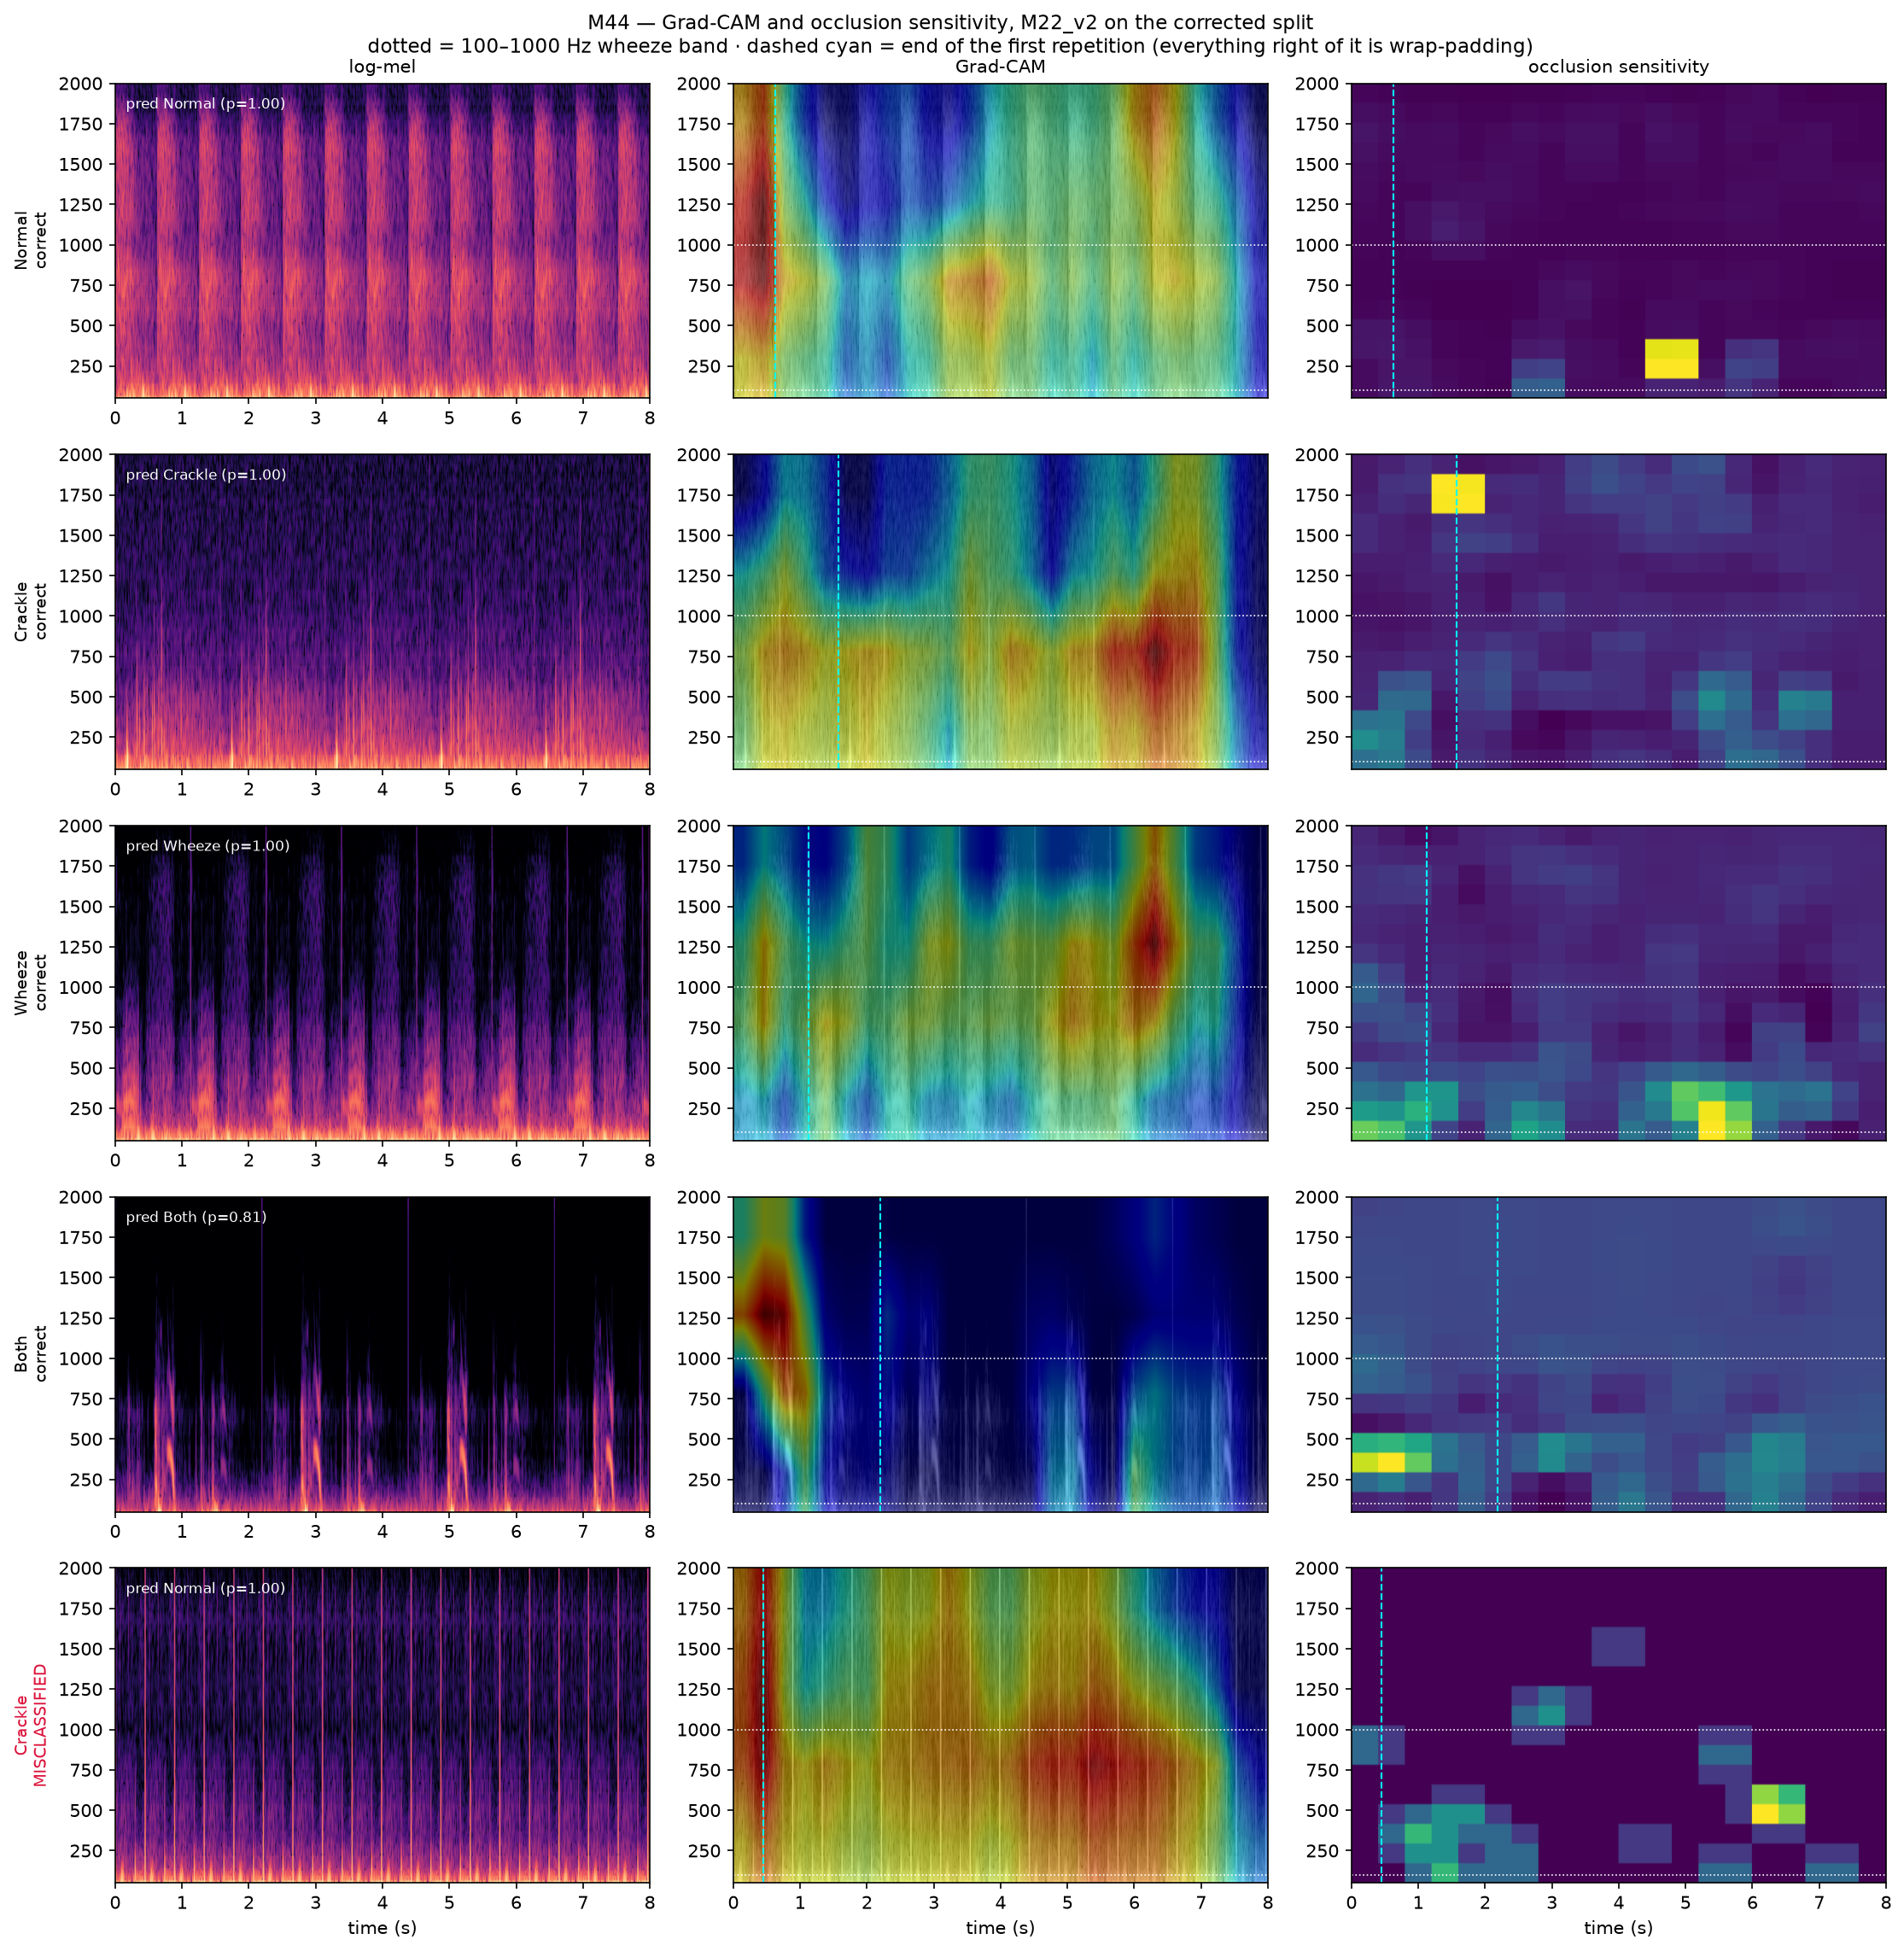
\includegraphics[width=0.42\linewidth]{figures/fig_xai_panels.png}
\caption{Attribution panels for the best model. Each row is one test cycle and shows the log-mel
spectrogram, the gradient-based attribution, the occlusion map, and the predicted against the
true label. The bottom row is a misclassified cycle.}
\label{fig:xai}
\end{figure}

\begin{table}[!t]
\centering
\caption{Quantitative explainability measurements on the best model over 400 test cycles. Band
pointing measures whether attribution concentrates in the 100 to 1000~Hz wheeze band, tiling
consistency measures whether the model attributes alike to the identical repeated copies of a
cycle inside one input, and padding attention measures how much attribution falls after the real
cycle ends.}
\label{tab:xaiquant}
\footnotesize
\begin{tabular}{llrl}
\toprule
Measure & Condition & Value & Reading \\
\midrule
\multirow{4}{*}{Band pointing}
 & uniform baseline & 0.5547 & what an unfocused map would give \\
 & wheeze absent ($n = 325$) & 0.7674 & concentrates in the band \\
 & wheeze present ($n = 75$) & 0.7140 & concentrates \emph{less} \\
 & \best{difference} & \best{$-0.0534$} & [$-$0.0785, $-$0.0256], $p = 0.001$ \\
\midrule
\multirow{3}{*}{Tiling consistency}
 & mean correlation ($n = 361$) & 0.098 & attribution differs across identical audio \\
 & median correlation & 0.180 & --- \\
 & fraction above 0.5 & 32.1\% & only a third are consistent \\
\midrule
\multirow{2}{*}{Padding attention}
 & cyclic tiling, observed / uniform & 0.594 / 0.679 & ratio 0.87 \\
 & zero padding, observed / uniform & 0.101 / 0.679 & ratio 0.15 \\
\bottomrule
\end{tabular}

\vspace{2pt}
\footnotesize MobileNetV2 downsamples by 32, so its final convolutional block is 4 frequency by
26 time cells, roughly 500~Hz and 0.31~s each, and every map in Fig.~\ref{fig:xai} is that grid
interpolated up to $128 \times 801$. The direction of both measurements can be trusted because
both intervals exclude their null, while the fine structure of the maps is interpolation and not
measurement. Where the two maps disagree, we prefer the occlusion map, since its grid is 16 mel
bins by 80 frames and it needs no gradient through a downsampled layer.
\end{table}

From the band-pointing block of Table~\ref{tab:xaiquant}, attribution concentrates in the 100 to
1000~Hz band for both groups, at 0.7674 when wheeze is absent and 0.7140 when wheeze is present,
against a uniform baseline of 0.5547. The difference of $-0.0534$ [$-$0.0785, $-$0.0256] at
$p = 0.001$ goes the wrong way for a wheeze detector, because the model looks at the
physiological band less when the target sound is actually there.

The tiling-consistency block reports a mean correlation of 0.098 and a median of 0.180 between
the attribution maps of the identical repeated copies of one cycle inside a single input, with
only 32.1 percent of cycles above 0.5. A model reading acoustics should attribute the same way
to every copy, so a big part of the attribution is following the position in the window instead
of the sound. This measurement is what made us add the zero-padding row \texttt{P4} of
Table~\ref{tab:ablation}. The padding-attention block shows the two input schemes behaving very
differently in the padded region, at a ratio of 0.87 for cyclic tiling against 0.15 for zero
padding. Replacing tiling with zero padding costs 0.0311, so tiling does carry information, and
these measurements do not settle whether that information is acoustic or positional.

We do not present any of this as clinical validation. The labels these attributions are aligned
to are reproduced by a physician at $\kappa = 0.035$ on crackles, as reported in
Section~\ref{subsec:human}, so a map aligned to them tells us where the model looks and not that
the model reasons the way a clinician does. One planned analysis is not reported, for the same reason.
A pointing game that asks whether attribution mass lands inside the annotated event window is
not defined on this corpus, because ICBHI annotates whether a cycle contains an adventitious
sound and not where it happens, and our pipeline crops to exactly that window, which fixes the
hit rate at 100 percent by construction.

\subsection{Comparison with Existing Works}
\label{subsec:comparison}

Table~\ref{tab:comparison} places this work against published systems on the same corpus. Every
row is given under the challenge metric of~(\ref{eq:official}), and the partition of every row is
named, because the argument of this paper is that a comparison missing those two columns is not a
comparison. Rows in different blocks sit on different partitions and are not rankable against one
another.

\begin{table}[!t]
\centering
\caption{Comparison against published systems on ICBHI 2017 under the challenge metric
of~(\ref{eq:official}). Blocks correspond to partitions and are not rankable against one another.
Area under the curve is omitted because none of the cited systems reports it for this four-class
task, and accuracy is given only where the source reports it; sensitivity, specificity and the
challenge score are the metrics this literature holds in common.}
\label{tab:comparison}
\footnotesize
\begin{tabular}{lllrrrr}
\toprule
Author & Dataset & Network & Acc. & $S_e$ & $S_p$ & \best{ICBHI} \\
\midrule
\multicolumn{7}{l}{\emph{Published 60/40 partition, directly comparable}}\\
Gairola \emph{et al.}~\cite{respirenet2021} & ICBHI 2017 & ResNet34, ImageNet & --- & 0.401 & 0.723 & 0.5620 \\
Moummad and Farrugia~\cite{scl2023} & ICBHI 2017 & CNN6, supervised contrastive & --- & 0.392 & 0.760 & 0.5755 \\
Niizumi \emph{et al.}~\cite{frozenfm2025} & ICBHI 2017 & M2D, frozen linear probe & --- & 0.466 & 0.722 & 0.5938 \\
Bae \emph{et al.}~\cite{bae2023patchmix} & ICBHI 2017 & AST, patch-mix contrastive & --- & 0.431 & 0.817 & 0.6237 \\
Kim \emph{et al.}~\cite{bts2024} & ICBHI 2017 & CLAP, text-aided & --- & 0.457 & 0.814 & 0.6354 \\
Jeong \emph{et al.}~\cite{pafa2025} & ICBHI 2017 & BEATs, patient-aware alignment & --- & 0.476 & 0.821 & \best{0.6484} \\
Tzeng \emph{et al.}~\cite{tzeng2025jmir} & ICBHI 2017 & seven senior physicians & --- & 0.232 & 0.723 & 0.4777 \\
\addlinespace
\best{This work} & ICBHI 2017 & MobileNetV2 + SpecAugment & --- & 0.456 & 0.672 & \best{0.5641} \\
\best{This work} & ICBHI 2017 & MobileNetV3-Small & --- & 0.198 & 0.828 & 0.5132 \\
\best{This work} & ICBHI 2017 & 2D-CNN from scratch & --- & 0.201 & 0.744 & 0.4720 \\
\midrule
\multicolumn{7}{l}{\emph{Corrected patient-independent partition, not comparable to the block above}}\\
\best{This work} & ICBHI 2017 & MobileNetV2 + SpecAugment & 0.5880 & 0.4089 & 0.7115 & \best{0.5602} \\
\best{This work} & ICBHI 2017 & Swin-T & 0.5649 & 0.3429 & 0.7179 & 0.5304 \\
\best{This work} & ICBHI 2017 & DeiT-S & 0.5554 & 0.2946 & 0.7353 & 0.5149 \\
\best{This work} & ICBHI 2017 & ViT-B/16, collapsed & 0.5910 & 0.0000 & 0.9987 & 0.4994 \\
\midrule
\multicolumn{7}{l}{\emph{Identifier-fallback partition, shown only to price the fault}}\\
This work & ICBHI 2017 & MobileNetV2 + SpecAugment & --- & 0.5696 & 0.7294 & 0.6495 \\
\bottomrule
\end{tabular}

\vspace{2pt}
\footnotesize The final block is not a result. It is the same model scored on the 11-patient
partition of Fault~2, reported so that the cost of that fault can be read against the published
literature: at 0.6495 it would have ranked second in the first block.
\end{table}

Read against the first block, this work sits with the ImageNet-pretrained convolutional systems
and below every system pretrained on audio. The four rows above 0.62 are all audio-pretrained,
which is the ordering the ablation of Section~\ref{subsec:ablation} predicts and the reason the
one audio-pretrained backbone in this study is the model whose absence is most costly. The
physician row is included because it is measured on the same labels under the same metric, and it
places the whole table in context: the reference standard this corpus is scored against is itself
reproduced by trained listeners at 0.4777.

The comparison also shows why the audit of Section~\ref{subsec:faults} matters for reading any
row in this table. The final block scores 0.6495 on a partition that is neither the published one
nor patient-independent, which would have placed it between two published systems. Nothing about
the model changed to produce it.

\section{Conclusions}
\label{sec:conclusion}

We set out to build an interpretable open-world respiratory sound classifier and ended up
building an audit. The turn came from a gate written down in advance: our concept detectors had
to reproduce ICBHI's crackle and wheeze labels above 0.65, they reached 0.5580 and 0.5340 over
two runs, and the rule said stop. Looking for an explanation sent us into our own evaluation
code, where we found five faults. A macro-averaged score variant inflated 20 runs by 0.0948 on
average; a split loader silently fell back to an 11-patient test set worth 0.0893; the published
split assigns recordings rather than patients, though repairing that leak is worth only 0.0039;
one recording's device suffix does not match the released audio; and selecting the checkpoint by
minimum loss rather than by the challenge score costs 0.0752 to 0.1015 across three seeds. Our
unaudited pipeline reported 0.7077 where the corrected one reports 0.5602, and that 0.1475 is
larger than every architectural choice in this paper put together.

Under the corrected protocol MobileNetV2 with spectrogram masking is our best model, at 0.5602
on the corrected partition and 0.5641 on the published one, with 2.2~M parameters. All three
vision transformers lost to it and ViT-B/16 collapsed to the majority class at 38 times the
parameter count, while the one audio-pretrained transformer cannot be placed beside them at all
because it predates the audit and stored no prediction table---the paper's own argument,
demonstrated on its own most interesting model. The ablation says fine-tuning is worth far more
than pretraining, that frozen ImageNet features are measurably \emph{worse} than random
projections on log-mel input, that masking buys specificity rather than sensitivity, and that
class weighting is worth less than the padding scheme---though a three-seed noise floor of
0.0141 rules three of those deltas inadmissible and a patient-level test over 47 patients
certifies only one. The concept branch ended in a retraction: a pre-registered probe on a frozen
AudioSet embedding reaches 0.7115 and 0.7621 on the very cycles our detectors failed on, so the
labels support strong detection and our extractors were weak. What replaced the claim is
better---on the same 132 clips that machine reproduces ICBHI's wheeze labels more closely than a
self-consistent physician does, by 0.169 at $p = 0.046$.

The practical recommendation is short. Report the challenge metric with sensitivity and
specificity beside it, name the partition and say whether it is patient-independent, commit the
raw confusion matrix, state the checkpoint selection rule, and test over patients rather than
cycles. Four of the five faults are invisible without those habits, all five sat in code that
ran without error, and the third is the one whose absence cost us an entire model.

Three directions follow from this work. \emph{A clean validation protocol, and the fourth
transformer re-run:} our harness monitors the test partition every epoch, so every score here
carries a selection advantage; carving a validation split from the 79 training patients would
remove that direct test-set selection advantage, and the audio-pretrained
transformer belongs in the same batch as the one experiment that tests the pretraining-domain
hypothesis directly. \emph{A reference standard built for the task:} a multi-rater re-annotation of even a few
hundred cycles, with calibration exemplars and an explicit ``fits no named category'' option,
would separate model error from label noise---our own pack found roughly 7 percent of clips
containing a sound fitting none of the four named classes.
\emph{Fine-tuning that preserves what pretraining learned:} the frozen probe in
Table~\ref{tab:ceiling} recovers these labels at 0.71 and 0.76 with no task training, while our
ImageNet backbones are useless until allowed to move. Whether adaptation can be constrained so
that it keeps the acoustic structure a large audio model already carries is a concrete next
step, and the probe supplies its success criterion.

Two habits underpin this work: fix the threshold before running the experiment, and audit
your own pipeline before you audit anyone else's.

%=======================================================================
\appendices
\section{Run Identifier Map}
\label{app:runmap}

Models are named by architecture throughout the paper. Each also carries a short internal
identifier, which names the result record every reported number was computed from.
Table~\ref{tab:runmap} maps one to the other so that each value above can be traced to its
source record.

\begin{table}[!htbp]
\centering
\caption{Internal run identifiers, the name used in this paper, and where each is reported.}
\label{tab:runmap}
\footnotesize
\begin{tabular}{lll}
\toprule
Identifier & Name in this paper & Reported in \\
\midrule
M22-v2 & MobileNetV2 + SpecAugment --- the reference and best model & Tables~\ref{tab:main}, \ref{tab:allruns} \\
M3-v2 & MobileNetV2, clean control, ablation row \texttt{C1} & Tables~\ref{tab:main}, \ref{tab:ablation} \\
M40, M41, M42 & ViT-B/16, Swin-T, DeiT-S & Tables~\ref{tab:main}, \ref{tab:efficiency} \\
M4 / M43 & AST pre-audit / its corrected re-run (\notrun) & Section~\ref{subsec:ast} \\
M1, M2, M3, M12, M22 & the pre-audit backbone line and its selection study & Table~\ref{tab:allruns}; Section~\ref{subsec:faults} \\
M7 & MobileNetV2 ensemble, $N = 5$ & Section~\ref{subsec:augmentation} \\
M6, M29 & OpenMax and post-hoc energy open-set baselines & Section~\ref{subsec:extensions} \\
M30--M37 & the extension sweep & Tables~\ref{tab:allruns}, \ref{tab:extensions} \\
M39 & physics-derived concept extraction and the gate & Table~\ref{tab:gate} \\
M44, M45 & interpretability analysis; component and preprocessing ablation & Tables~\ref{tab:xaiquant}, \ref{tab:ablation} \\
M48 & protocol ablation, seed band, same-clips comparison & Tables~\ref{tab:human}, \ref{tab:stats}; Table~\ref{tab:protocol} \\
N11 & supervised ceiling estimate & Table~\ref{tab:ceiling} \\
\bottomrule
\end{tabular}
\end{table}

%=======================================================================
\bibliographystyle{IEEEtran}
\bibliography{references}

\end{document}
